\documentclass[a4paper, 12pt]{article}

% Margins
\topmargin=-0.45in
\evensidemargin=0in
\oddsidemargin=0in
\textwidth=6.5in
\textheight=9.0in
\headsep=0.25in 

%package usage
\PassOptionsToPackage{svgnames}{xcolor}
\usepackage[colorlinks=true, citecolor=blue, linkcolor=purple]{hyperref}
\usepackage[english]{babel}
\usepackage[latin1]{inputenc}
\usepackage{enumitem}
\usepackage{indentfirst}
\usepackage{colortbl}
\usepackage{longtable}
\usepackage{animate}
\usepackage{threeparttablex}
\usepackage{etoolbox}
\usepackage{rotating}
\usepackage{multirow}
\usepackage{pdflscape}
\usepackage{tablefootnote}
\usepackage[table,xcdraw]{xcolor}
\usepackage{amsmath}
\usepackage{flafter} 
\usepackage{dcolumn} 
\usepackage{natbib}
\usepackage{rotating}	
\usepackage{adjustbox}
\usepackage{amsthm}
\usepackage{graphicx}
\usepackage{amssymb}
\usepackage{tcolorbox}
\usepackage{lipsum}
\usepackage{tikz}
\usepackage{tabularx}
\tcbuselibrary{skins,breakable}
\usetikzlibrary{shadings,shadows}
\usepackage{threeparttable}
\usepackage{subfig}
\usepackage{setspace}
\usepackage{booktabs}
\usepackage{placeins}
\usepackage{enumitem}
\usepackage{natbib}
\usepackage{filecontents}
\usepackage[encoding,filenameencoding=utf8,extendedchars,space]{grffile}
\newcommand{\addfig}[2]{\begin{center}
			\includegraphics[width=#1\textwidth]{#2}
	\end{center}
}

%\usepackage[capposition=top]{floatrow}
%\usepackage[colorinlistoftodos]{todonotes}
\newcommand{\expect}[2]{\mathbb{E}_{#2}\left(#1\right)}

\newtheorem{theorem}{Theorem}[section]
\newtheorem{corollary}{Corollary}[theorem]
\newtheorem{proposition}[theorem]{Proposition}

\newcommand{\alert}[1]{{\textbf{\color{red}#1}}}
%general commands

\newcommand{\bcite}{\begin{quote}}
\newcommand{\ecite}{\end{quote}}
\newcommand{\beqns}{\begin{eqnarray*}}
\newcommand{\eeqns}{\end{eqnarray*}}
\newcommand{\beqn}{\begin{eqnarray}}
\newcommand{\eeqn}{\end{eqnarray}}
\newcommand{\benu}{\begin{enumerate}}
\newcommand{\eenu}{\end{enumerate}}
\newcommand{\bitem}{\begin{itemize}}
\newcommand{\eitem}{\end{itemize}}
\newcommand{\smallGap}{\vspace{.25cm}}

\newenvironment{block}[1]{%
	\tcolorbox[beamer,%
	noparskip,breakable,
	colback=LightGreen,colframe=DarkGreen,%
	colbacklower=LimeGreen!75!LightGreen,%
	title=#1]}%
{\endtcolorbox}


\newcommand{\sym}[1]{\rlap{#1}}% Thanks David Carlisle

\usepackage{siunitx}
\sisetup{
	detect-mode,
	group-digits		= false,
	input-symbols		= ( ) [ ] - +,
	table-align-text-post	= false,
	input-signs             = ,
}

%mathematical commands
\newcommand{\problemIndustries}{(A_t\cup \Omega_t)}
\newcommand{\red}[1]{{\color{red}#1}}
\newcommand{\normalIndustries}{\problemIndustries^C}
\newcommand{\sumNormalIndustries}{\sum_{j\in\normalIndustries}}
\newcommand{\sumProblemIndustries}{\sum_{j\in\problemIndustries}}
\newcommand{\sumWithinNormal}{\sum_{j\in\normalIndustries\cap \Gamma_t}}
\newcommand{\sumWithinProblem}{\sum_{j\in\normalIndustries\cap \Gamma_t^C}}
\newcommand{\ser}[1]{s_{er#1}}
\newcommand{\cov}{\text{cov}}
\newcommand{\explain}[2]{\underbrace{#1}_{\parbox{\widthof{\ensuremath{#1}}}{\footnotesize\raggedright #2}}}
\newcommand{\lfpthresh}[1]{\underline{\chi_{#1 lt}}}
\newcommand{\crho}{\frac{\sigma-1}{\sigma}}
\newcommand{\crhoinv}{\frac{\sigma}{\sigma-1}}

\newcommand{\lquote}[3][]{\bcite #2 \citep[#1]{#3} \ecite}

\newcommand{\laquote}[3][]{\bcite #2 \citepalias[#1]{#3} \ecite}
\usepackage{tabularx}
\defcitealias{NationalAcademyofSciences.CommitteeonOccupationalClassificationandAnalysis.1971}{National Academy of Sciences, 1971}


\title{Code documentation}
\author{C\'esar Garro-Mar\'in\thanks{Boston University, email: \href{mailto:cesarlgm@bu.edu}{cesarlgm@bu.edu}}} 

\begin{document}
\maketitle

%
%\section{A refresher on GMM}
%
%In GMM we consider parameters that are defined by a set of orthogonality conditions:
%\beqns
%	\expect{\psi(w,\theta)}{}=0
%\eeqns
%where 
%\bitem
%	\item $w$ is a $p$ random vector
%	\item $\psi$ is a $r\times 1$ vector of functions.
%	\item $\theta$ is a $k\times 1$ vector of unknown parameters.
%\eitem 
%
%We have a sample of $N$ observations. GMM estimation is based in minimizing the quadratic form:
%\beqns
%\hat{\theta}=\text{argmin}_{c\in \Theta} b_N(c)'A_Nb_N(c)
%\eeqns
%where
%\beqns
%b_N(c)=\frac{1}{N}\sum_{n=1}^N\psi(w_n,c)
%\eeqns
%
%\section{Translating to the problem at hand:}
%Let 
%\beqns
%	\sigma&=&\left(\sigma_1, \dots, \sigma_J\right)	\\
%	\theta&=&\left(\theta_1^l, \theta_2^l \dots \theta_4^h\right) \\
%   \Lambda&=&\left(\Delta \ln A_{1t}^l, \Delta \ln A_{2t}^l, \Delta \ln
%   A_{3t}^l,\Delta \ln A_{1t+1}^l \dots \Delta \ln A_{3T}^h\right)
%\eeqns


\section{New approach (v2):}
\subsection{Model equations}
At the job level it holds that:
\beqn
\Delta \overline{ \ln S^e_{iJet}}&=&\frac{\sigma_J}{\sigma_J-1} \left(\sum_k \theta_k^e\overline{S_{keJt}} \Delta \ln A_{kJt}-\Delta \ln A_{iJt}\right) \label{eq:skills_eq} \\ 
\Delta \overline{ \ln S^e_{iJet}}-\Delta \overline{ \ln S^e_{kJet}}&=&\frac{\sigma_J}{\sigma_j-1}\left(\Delta \ln
A_{kJt}-\Delta \ln A_{iJt} \right)  \label{eq:pi_equation} \\ 
1&=&\sum_k\theta_k^e\overline{S_{keJt}}  \label{eq:total_sum} \\  
\Delta  \left[\ln \frac{q_{eJt}}{q_{e'Jt}}\right]&=&\sum_k\left(\theta_k^e \overline{S_{kJet}}-\theta_k^{e'} \overline{S_{kJe' t}}\right)\Delta \ln A_{kjt}+const_{e,e't} \label{eq:employment_eq} 
\eeqn
\paragraph*{Note:} in equation \eqref{eq:employment_eq} there is always a
redundant pairwise comparison. Note that $\Delta  \left[\ln
\frac{q_{eJt}}{q_{e'Jt}}\right]-\Delta  \left[\ln \frac{q_{e'Jt}}{q_{e^\star
Jt}}\right]=\Delta  \left[\ln
\frac{q_{eJt}}{q_{e^\star Jt}}\right]$

\subsection{Building GMM}
In our data we have 3 education levels, 4 skills, $J$ jobs and $T$ periods.
\bitem
	\item \textbf{Equation (1)}: 
	Let $x_{ejt}$ be the row vector $\begin{pmatrix}
		S_{1ejt}&S_{2ejt}&S_{3ejt}&S_{4ejt}
	\end{pmatrix}$.  Define the matrix $X_{ejt}$ as the 4$\times$4 matrix containing the skill indexes by education. For simplicity, I have ignored the bars in the notation.
	\beqns
		X_{ejt}&=&\begin{pmatrix}S_{1ejt}&S_{2ejt}&S_{3ejt}&S_{4ejt}\\
							S_{1ejt}&S_{2ejt}&S_{3ejt}&S_{4ejt}\\
							S_{1ejt}&S_{2ejt}&S_{3ejt}&S_{4ejt}\\
							S_{1ejt}&S_{2ejt}&S_{3ejt}&S_{4ejt}\\
		\end{pmatrix}=\begin{pmatrix}
		x_{ejt} \\
		x_{ejt}\\
		x_{ejt}\\
	x_{ejt}	\end{pmatrix}
	\eeqns
	Let $X$ be the matrix stacking all the $X_{ejt}$ in some order that for now is irrelevant. The only thing that matters is that I use the same order across all definitions. This matrix is of dimension $N\times4$.
	\beqns
		X&=&\begin{pmatrix}	X_{111} \\\
		\vdots \\\
	 X_{3JT}\end{pmatrix}
	\eeqns
 	Let $I_e$ be the $N\times4$ matrix with columns given by education level $e$ dummies:
 	\beqns
 		I_e&=&\begin{pmatrix}\iota_e&\iota_e&\iota_e&\iota_e\end{pmatrix}
 	\eeqns
 	The set of instruments for equation 1 is then:
 	\beqn
 	 		Z_1&=&\begin{pmatrix}I_1\odot X& I_2\odot X &I_3\odot X \end{pmatrix} \label{eq:equation1Z}
	\eeqn
	\item \textbf{Equation \eqref{eq:pi_equation}}: set of instruments are a set of
	occupation by year doummies $Z_2$.
	\item \textbf{Equation \eqref{eq:total_sum}}: let $\tilde{X_e}$ be the $N_e\times 4$ matrix stacking all the $x_{ejt}$ for education level $e$. The instruments for equation 2 are the block diagonal matrix with elements $\tilde{X_e}$:
	\beqns
		Z_3&=&\begin{pmatrix}
			\tilde{X_1} & 0 &0 \\
			0 & \tilde{X_2} & 0 \\
			0 & 0 &\tilde{X_3}
		\end{pmatrix}
	\eeqns
	\item \textbf{Equation \eqref{eq:employment_eq}} let $\bar{X}$ be the matrix stacking the row vectors $\begin{pmatrix}x_{1jt}&x_{2jt}&x_{3jt}\end{pmatrix}$. Let $C$ be the matrix containing education-pair$\times$T dummies. Instruments for equation 3 are:
	\beqn
		Z_4&=&\begin{pmatrix}
			\bar{X} & C
		\end{pmatrix}
	\eeqn
	\item \textbf{Putting it all together:} let $u_l$ be the stacked (in the appropriate order) vector of equation $l$ errors. Define:
	\beqns
		Z'&=&\begin{pmatrix}
			Z_1' & 0 & 0  & 0\\
			0 & Z_2' & 0 & 0 \\
			0 & 0 & Z_3' & 0 \\
			0 & 0 & 0 & Z_4' \\	
	\end{pmatrix}\\
		u&=&\begin{pmatrix}
		u_1\\ u_2 \\ u_3 \\ u_4
		\end{pmatrix}
	\eeqns
	the moment equations form the model are given by $\expect{Z'u}{}=0$.
\eitem 
\section{How did I write the code?}
\subsection{Basic definitions}
\beqns
	\Lambda&=&\begin{pmatrix}
		\Delta \ln A_{111} \\
		\Delta \ln A_{121} \\
		\Delta \ln A_{131} \\
		\vdots \\
			\Delta \ln A_{3JT-2} \\
		\Delta \ln A_{3JT-1} \\
		\Delta \ln A_{3JT} \\
	\end{pmatrix}\text{\vspace{1cm}}
	\Theta=\begin{pmatrix}
	 \theta_{1}^1 \\
	\theta_{2}^1\\
	\theta_{3}^1 \\
	\theta_{4}^1\\
	\vdots \\
	\theta_{1}^3 \\
	\theta_{2}^3\\
	\theta_{3}^3 \\
	\theta_{4}^3
\end{pmatrix} \Sigma=\begin{pmatrix}
\sigma_1 \\
\vdots \\
\sigma_J
\end{pmatrix} \Xi = \begin{pmatrix}
	\xi_{11} \\
	\vdots \\
	\xi_{3T}
\end{pmatrix}
\eeqns
I defined the model parameter vector as
\beqns
	\Pi=\begin{pmatrix}
		\Lambda \\
		\Theta \\
		\Sigma \\
		\Xi 
	\end{pmatrix}
\eeqns
\subsection{Equation \eqref{eq:pi_equation}}
\benu
	\item Order observations by skill, education, occupation, and year.
	\item Create vector $\tilde{\Sigma}$
	\beqns
		\tilde{\Sigma}=\begin{pmatrix}
			\sigma_1\\
			\sigma_2\\
			\vdots\\
			\sigma_J
		\end{pmatrix}
	\eeqns
	this vector of is has the same dimensions as $\Lambda$. It places all elements of $\Sigma$ in the ``right'' order \red{I should say what the right order is here}.
	\item Define $D$ as a matrix of dimensions $(E\times J \times T)\times(J\times T)$. Define $Z_1$ as:
	\beqns
		X_1&=&\begin{pmatrix}
			-D & 0 &0 \\
			0 & -D &0 \\
			0 & 0 &-D \\
		\end{pmatrix}
	\eeqns
	This matrix contains occupation by year dummies. Equation \eqref{eq:pi_equation} can be written as:
	\beqns
		y_1=X_1\times (\Lambda\odot \tilde{\Sigma})
	\eeqns
	where $y_1$ was defined in the appropriate order.
\eenu

%
%\subsection{What are the new estimates of $\theta_{jt}$}
%\begin{table}[htbp]\centering \caption{$\theta_{ie}$ estimates} \begin{tabular}{l*{4}{c}} \toprule
            &      manual&     routine&      social&    abstract\\
\midrule
Low         &        0.46&        0.40&        0.37&        0.64\\
Mid         &        0.65&        0.29&        0.20&        0.67\\
High        &        0.59&        0.45&        0.25&        0.61\\
\bottomrule
\end{tabular}
\end{table}

%
%\subsection{How do the $\pi_{jt}$ look like?}
%$\pi_{jt}$ are simple occupation-year averages:
%\beqns
%	\hat{\pi}_{jt}=\sum_e	\left(\Delta \ln S_{ijet}-\Delta \ln S_{1ket}\right)
%\eeqns
%$\Rightarrow$  any difference across education groups comes from occupational distribution.
%
%\begin{table}[htbp]\centering
\def\sym#1{\ifmmode^{#1}\else\(^{#1}\)\fi}
\caption{Variation of $\pi\_{jt}$, baseline. pooled}
\begin{tabular}{l*{1}{cccc}}
\toprule
                    &\multicolumn{1}{c}{(1)}&            &            &            \\
                    &        mean&          sd&         p25&         p75\\
\midrule
Routine             &       -0.00&        0.15&       -0.09&        0.09\\
pi\_manual           &        0.01&        0.13&       -0.07&        0.09\\
Social              &        0.00&        0.09&       -0.04&        0.04\\
\midrule
Observations        &        3948&            &            &            \\
\bottomrule
\end{tabular}
\end{table}

%\begin{table}[htbp]\centering
\def\sym#1{\ifmmode^{#1}\else\(^{#1}\)\fi}
\caption{Variation of $\pi_{jt}$, baseline, 2000-2017}
\begin{tabular}{l*{1}{cccc}}
\toprule
                    &\multicolumn{1}{c}{(1)}&            &            &            \\
                    &        mean&          sd&         p25&         p75\\
\midrule
Routine             &       -0.01&        0.14&       -0.09&        0.07\\
pi\_manual           &        0.01&        0.13&       -0.06&        0.10\\
Social              &        0.01&        0.09&       -0.04&        0.06\\
\midrule
Observations        &        1304&            &            &            \\
\bottomrule
\end{tabular}
\end{table}

%\begin{table}[htbp]\centering
\def\sym#1{\ifmmode^{#1}\else\(^{#1}\)\fi}
\caption{Variation of $\pi_{jt}$, squares, pooled}
\begin{tabular}{l*{1}{cccc}}
\toprule
                    &\multicolumn{1}{c}{(1)}&            &            &            \\
                    &        mean&          sd&         p25&         p75\\
\midrule
Routine             &       -0.00&        0.15&       -0.09&        0.08\\
pi\_manual           &        0.01&        0.14&       -0.07&        0.09\\
Social              &        0.00&        0.10&       -0.06&        0.05\\
\midrule
Observations        &        3948&            &            &            \\
\bottomrule
\end{tabular}
\end{table}

%\begin{table}[htbp]\centering
\def\sym#1{\ifmmode^{#1}\else\(^{#1}\)\fi}
\caption{Variation of $\pi_{jt}$, squares, 2000-2017}
\begin{tabular}{l*{1}{cccc}}
\toprule
                    &\multicolumn{1}{c}{(1)}&            &            &            \\
                    &        mean&          sd&         p25&         p75\\
\midrule
Routine             &       -0.01&        0.14&       -0.09&        0.07\\
pi\_manual           &        0.01&        0.14&       -0.08&        0.12\\
Social              &        0.01&        0.11&       -0.05&        0.06\\
\midrule
Observations        &        1304&            &            &            \\
\bottomrule
\end{tabular}
\end{table}

%
%\section{Exploring the scales}
%\begin{figure}[!h]
\centering
\caption{title}
\label{fig:key}
\subfloat[Pooled]{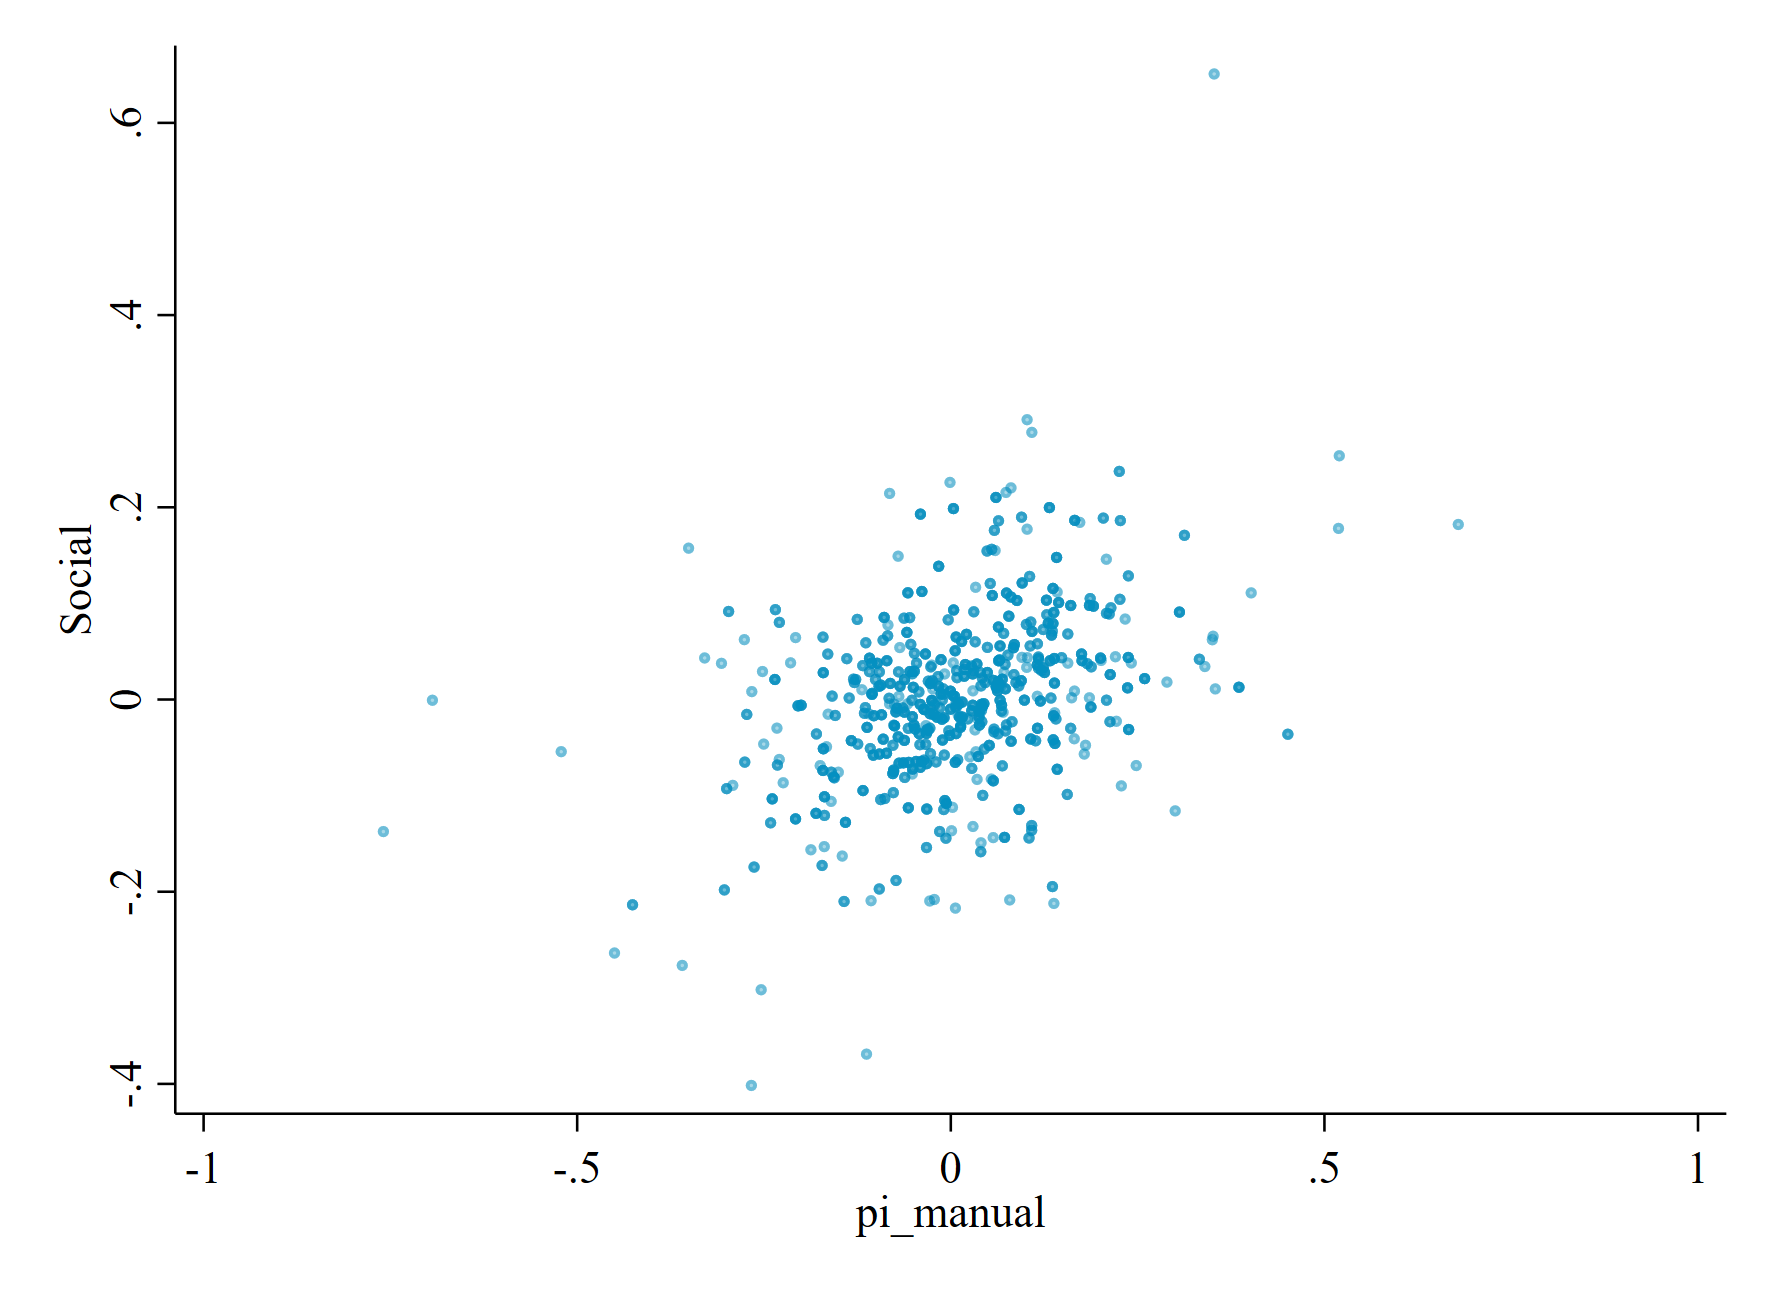
\includegraphics[width=.5\textwidth]{../results/figures/pi_social_pooled}} \subfloat[2000-2017]{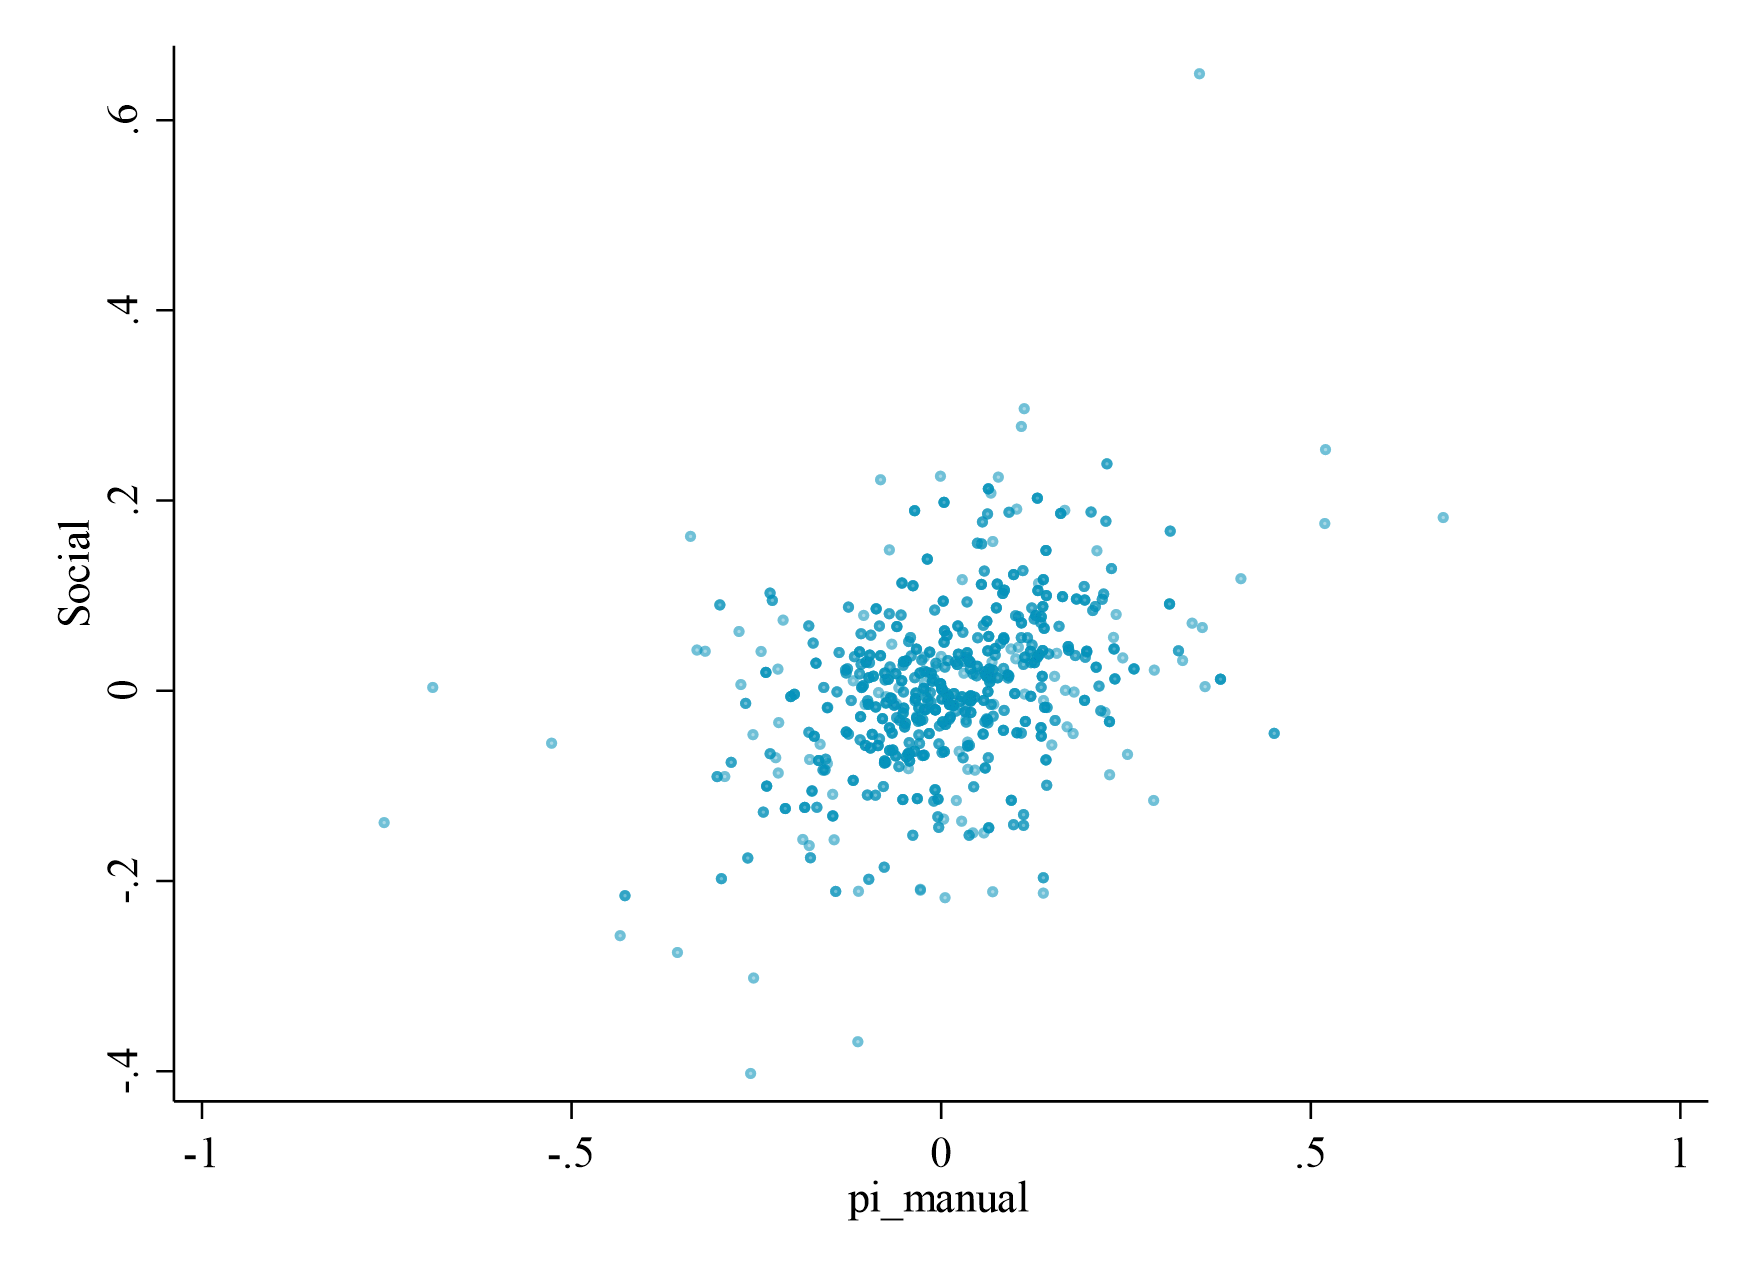
\includegraphics[width=.5\textwidth]{../results/figures/pi_social_all}} \\ \subfloat[Pooled]{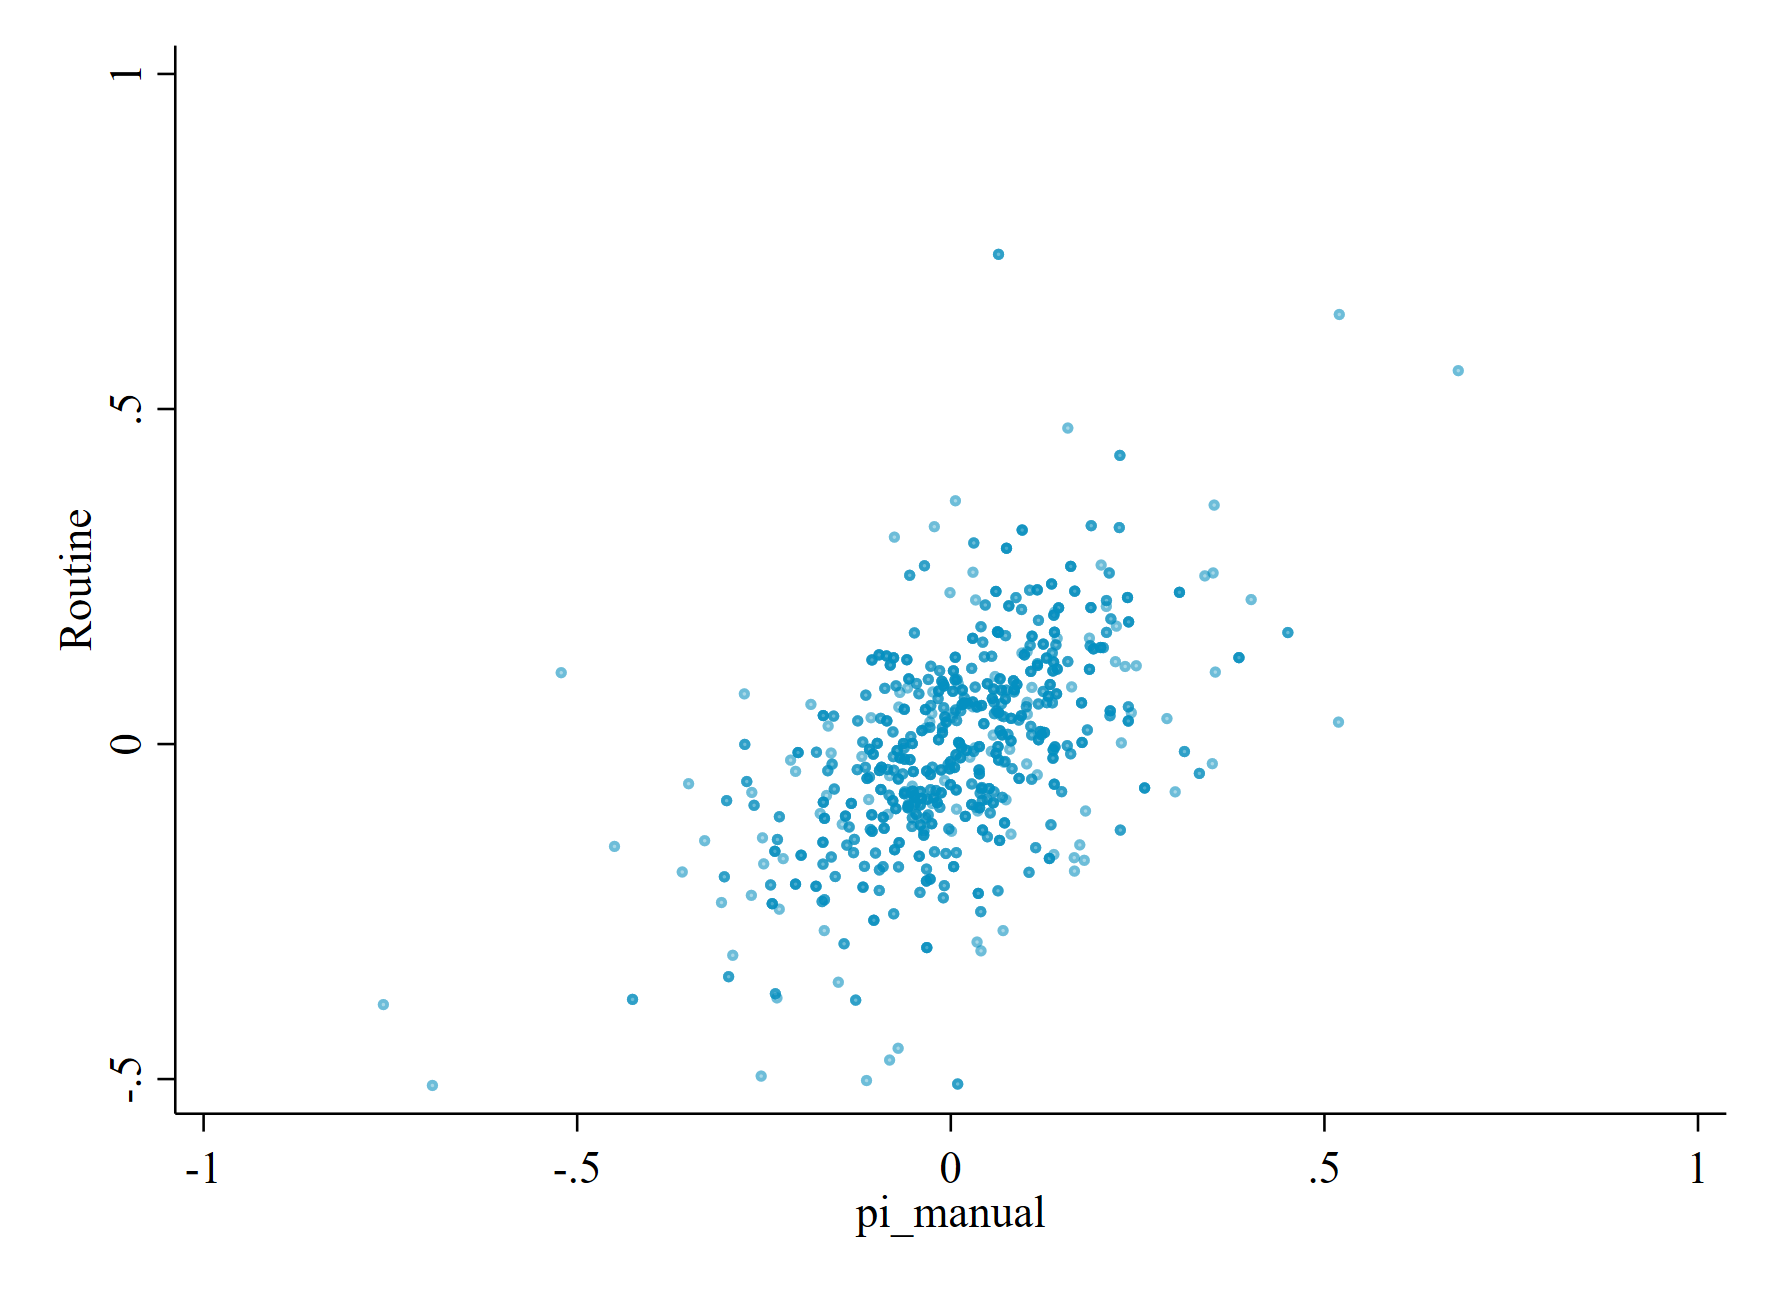
\includegraphics[width=.5\textwidth]{../results/figures/pi_routine_pooled}} \subfloat[2000-2017]{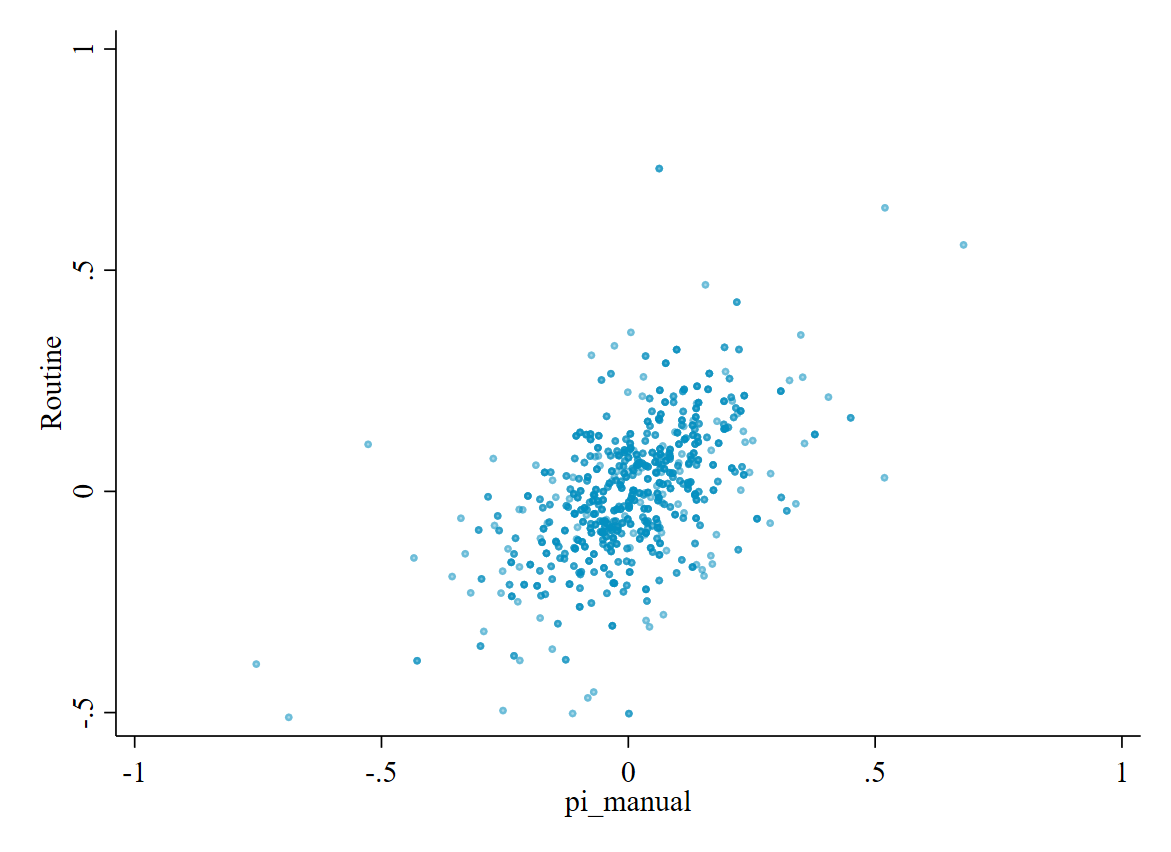
\includegraphics[width=.5\textwidth]{../results/figures/pi_routine_all}} \\ 
\par \begin{minipage}[h]{\textwidth}{\scriptsize\textbf{Note:} figure note. Figure generated on  3 May 2022 at 10:08:45.}\end{minipage}
\end{figure}

%\FloatBarrier
%\begin{figure}[!h]
\centering
\caption{Answer 100}
\subfloat[]{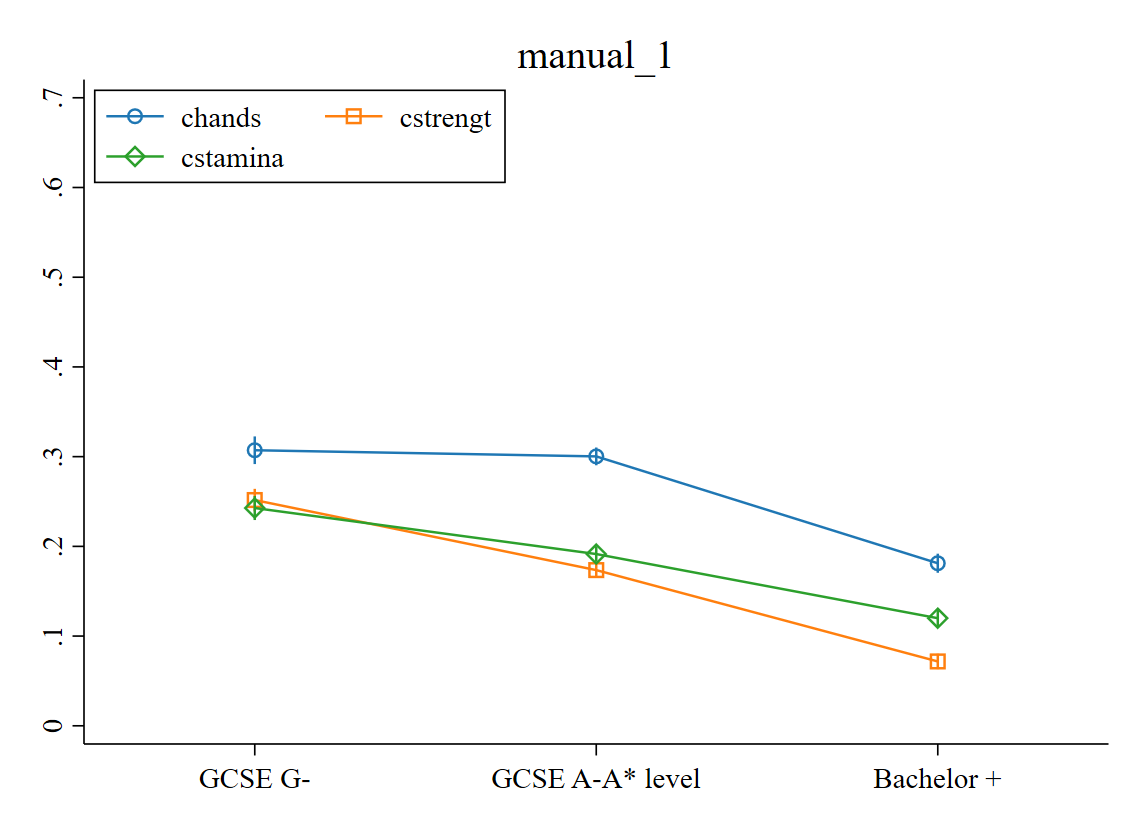
\includegraphics[width=.5\textwidth]{../results/figures//manual_100}} \subfloat[]{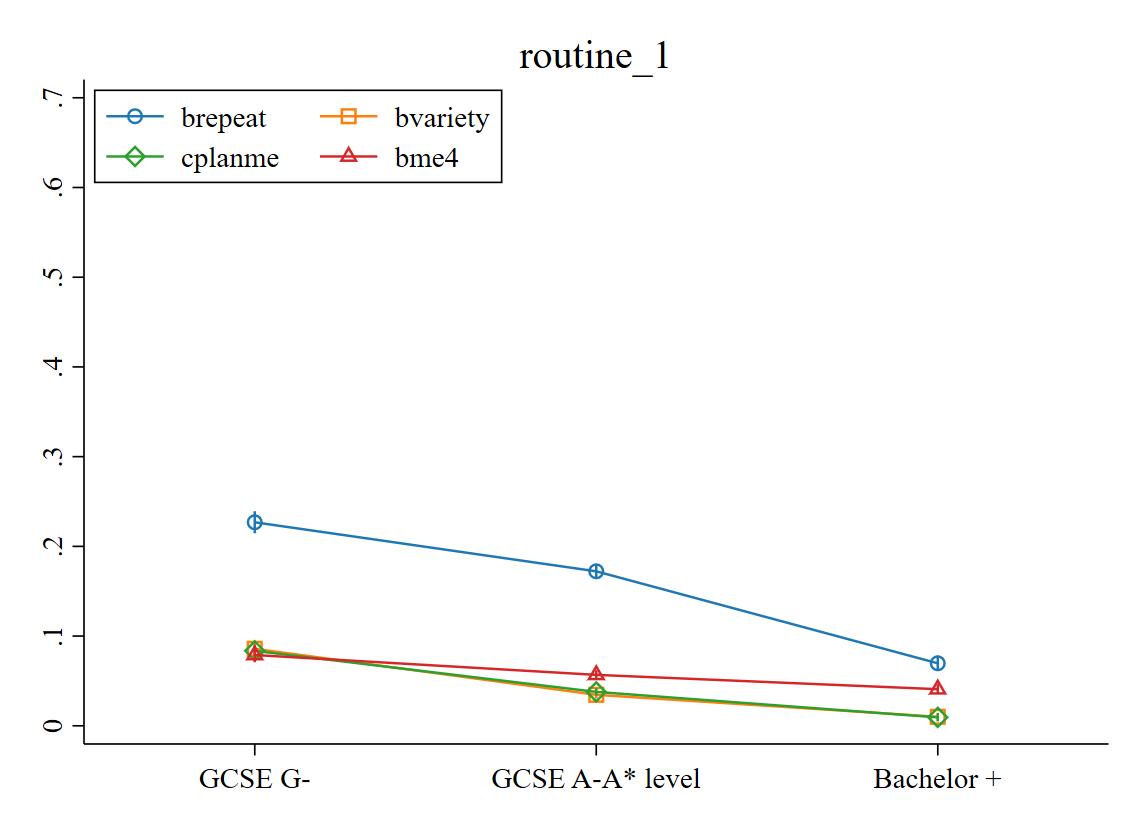
\includegraphics[width=.5\textwidth]{../results/figures//routine_100}} \\ \subfloat[]{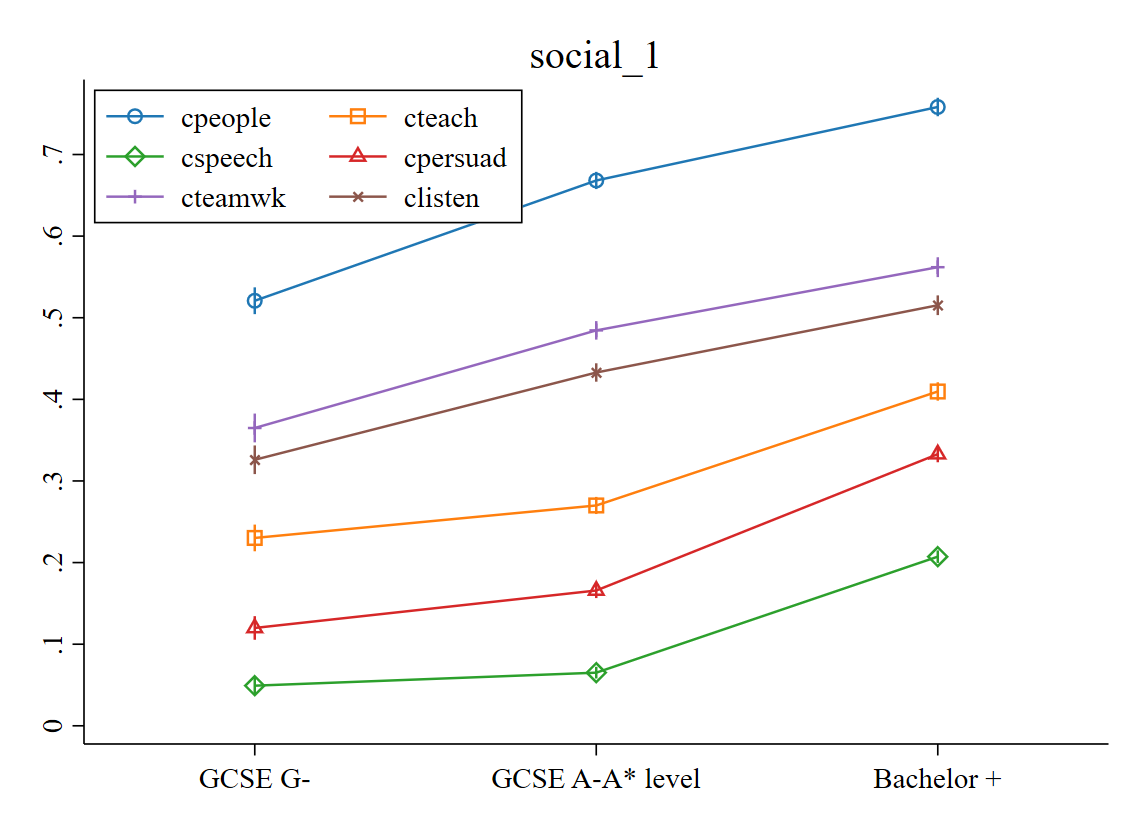
\includegraphics[width=.5\textwidth]{../results/figures//social_100}} \subfloat[]{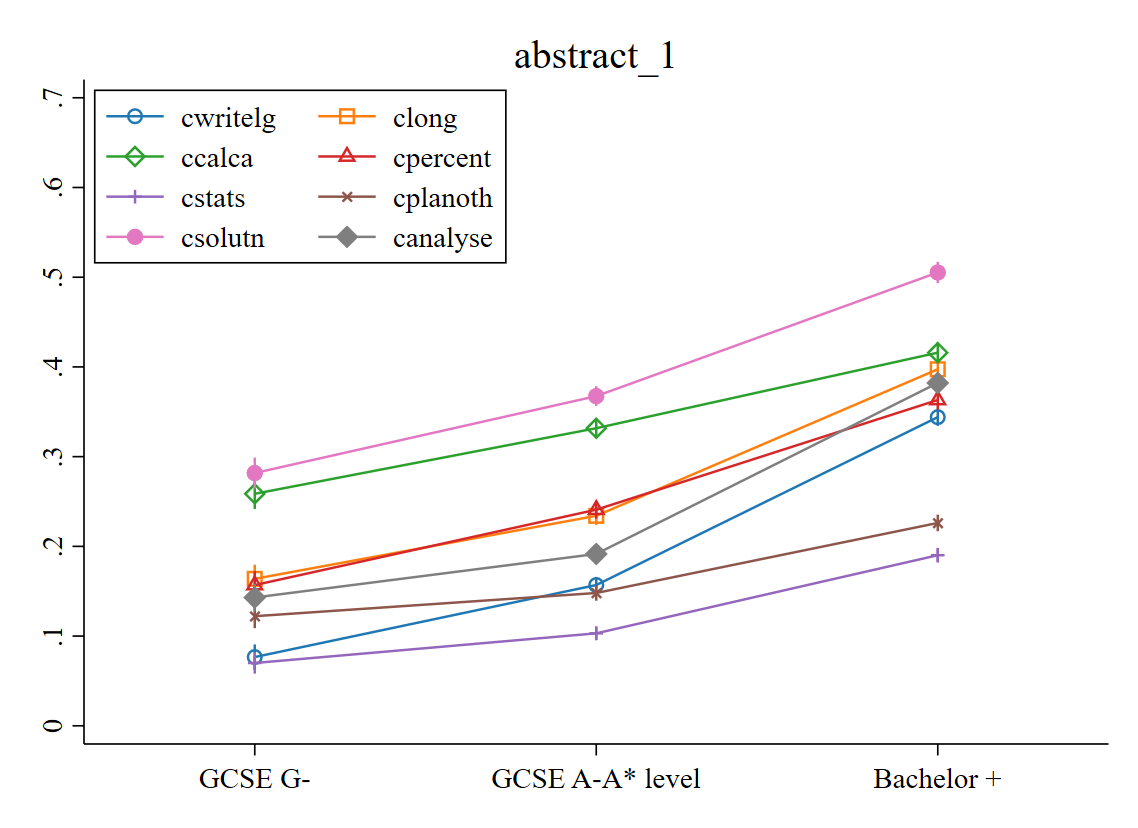
\includegraphics[width=.5\textwidth]{../results/figures//abstract_100}} \\ 
\end{figure}

%\begin{figure}[!h]
\centering
\caption{Answer 75}
\subfloat[]{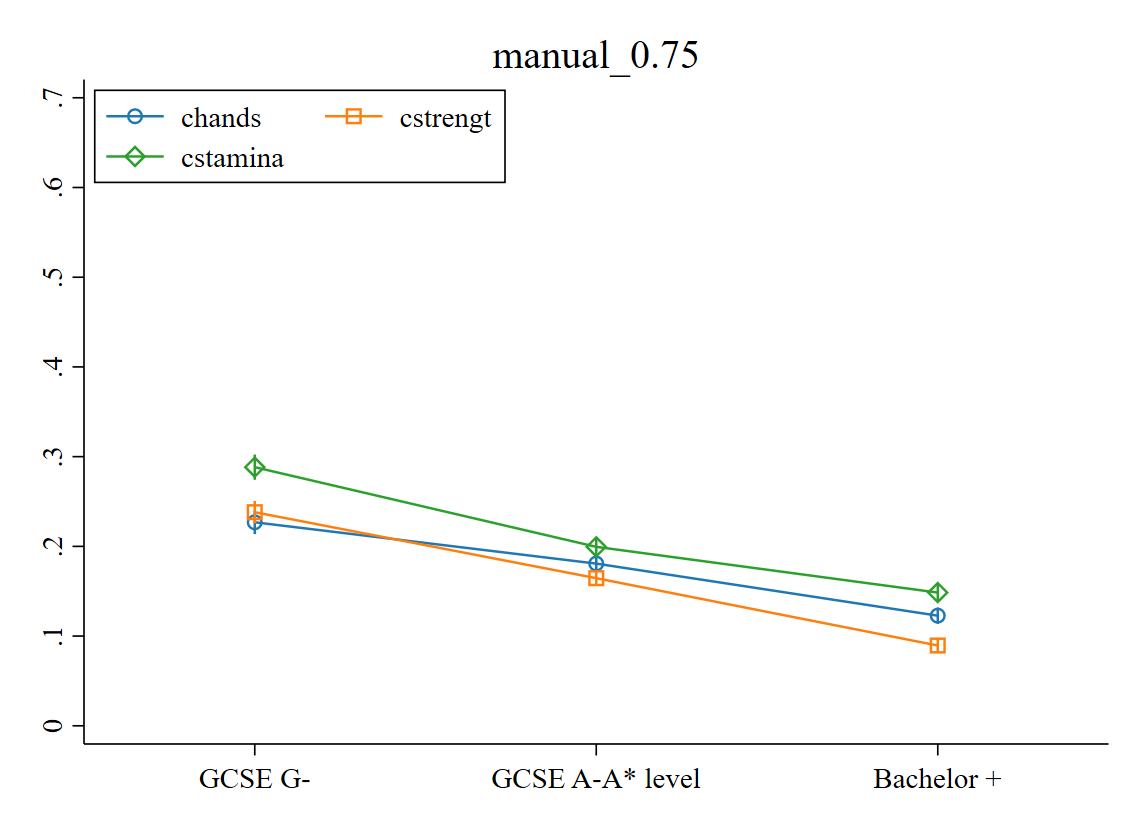
\includegraphics[width=.5\textwidth]{../results/figures//manual_75}} \subfloat[]{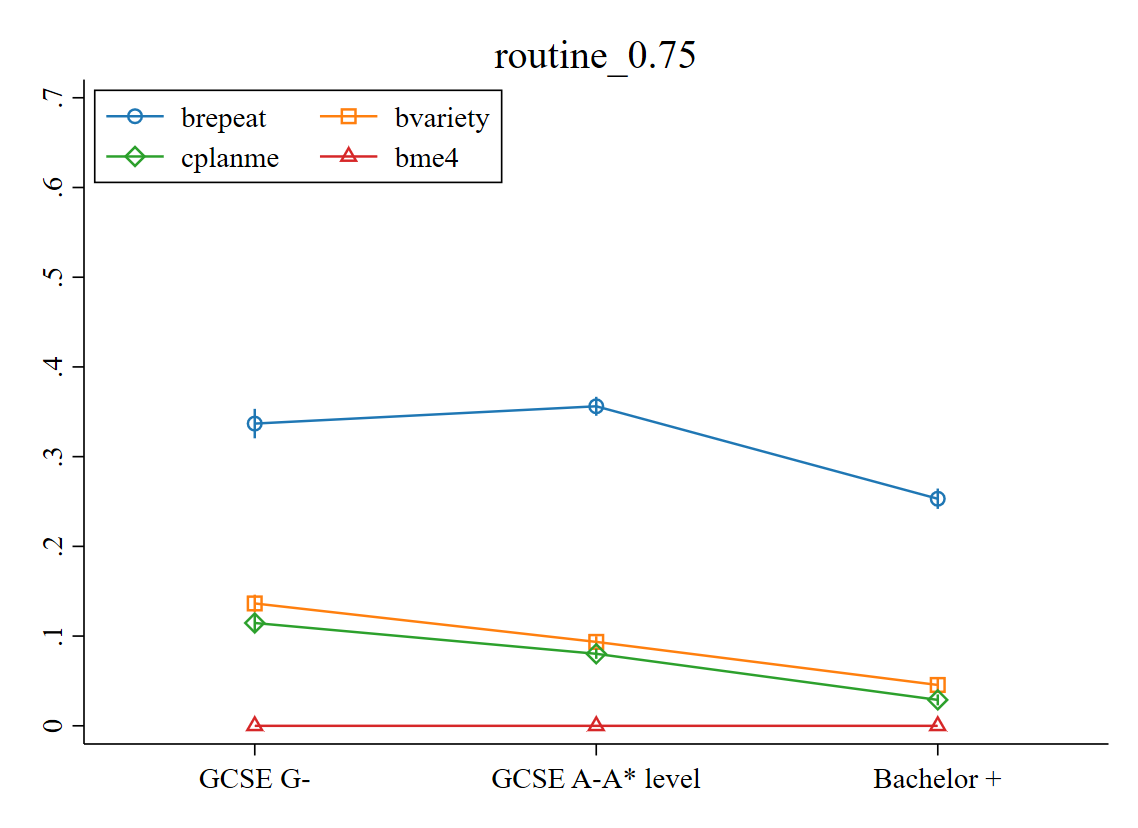
\includegraphics[width=.5\textwidth]{../results/figures//routine_75}} \\ \subfloat[]{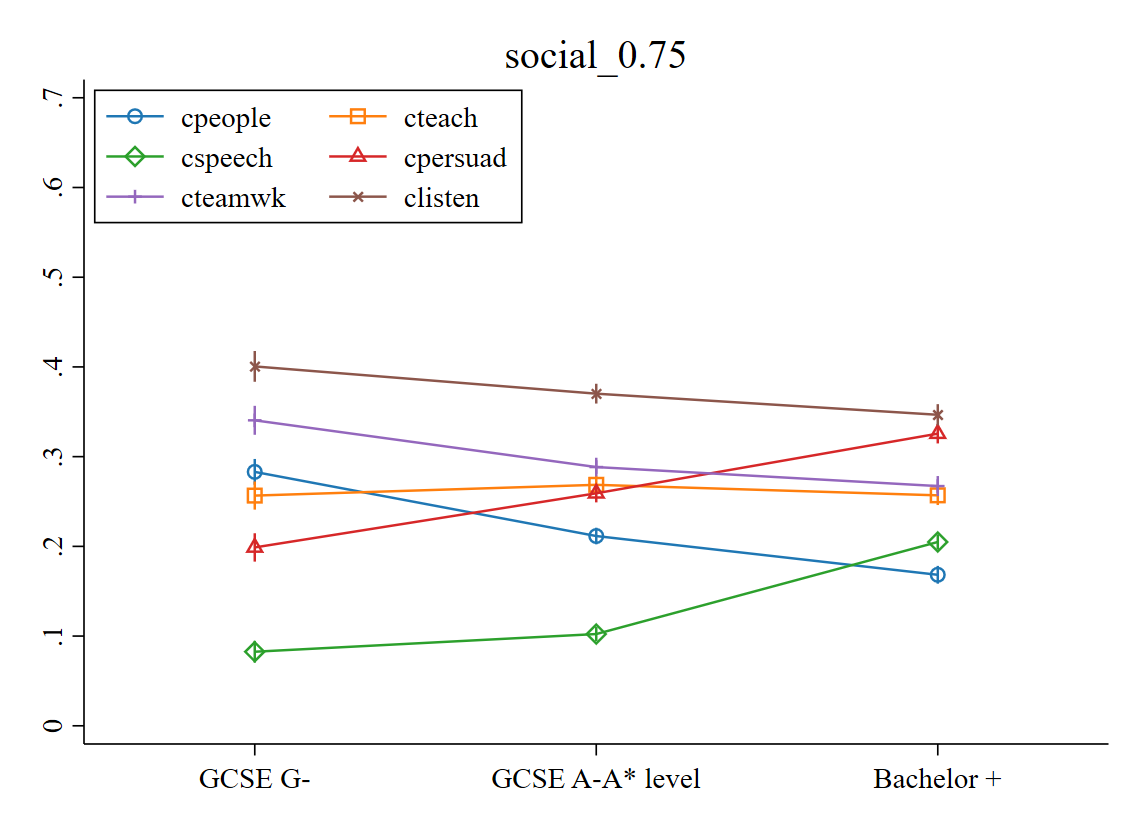
\includegraphics[width=.5\textwidth]{../results/figures//social_75}} \subfloat[]{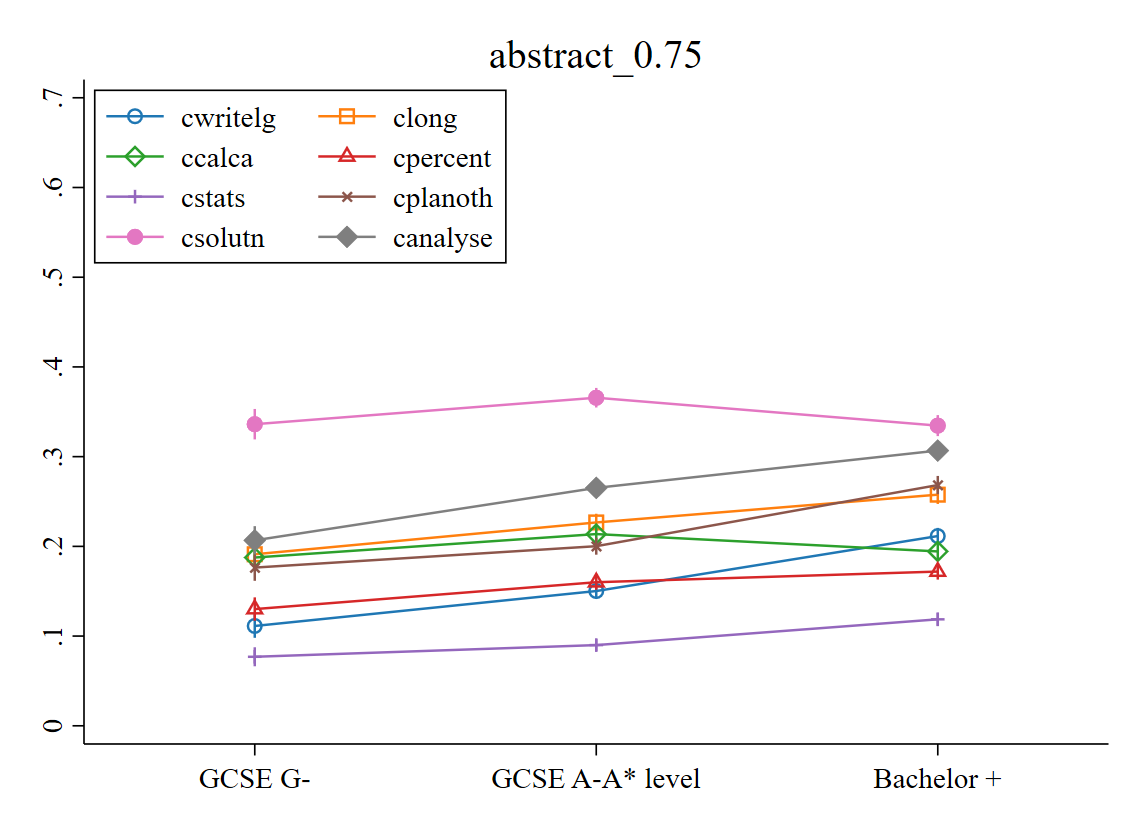
\includegraphics[width=.5\textwidth]{../results/figures//abstract_75}} \\ 
\end{figure}

%\begin{figure}[!h]
\centering
\caption{Answer 25}
\subfloat[]{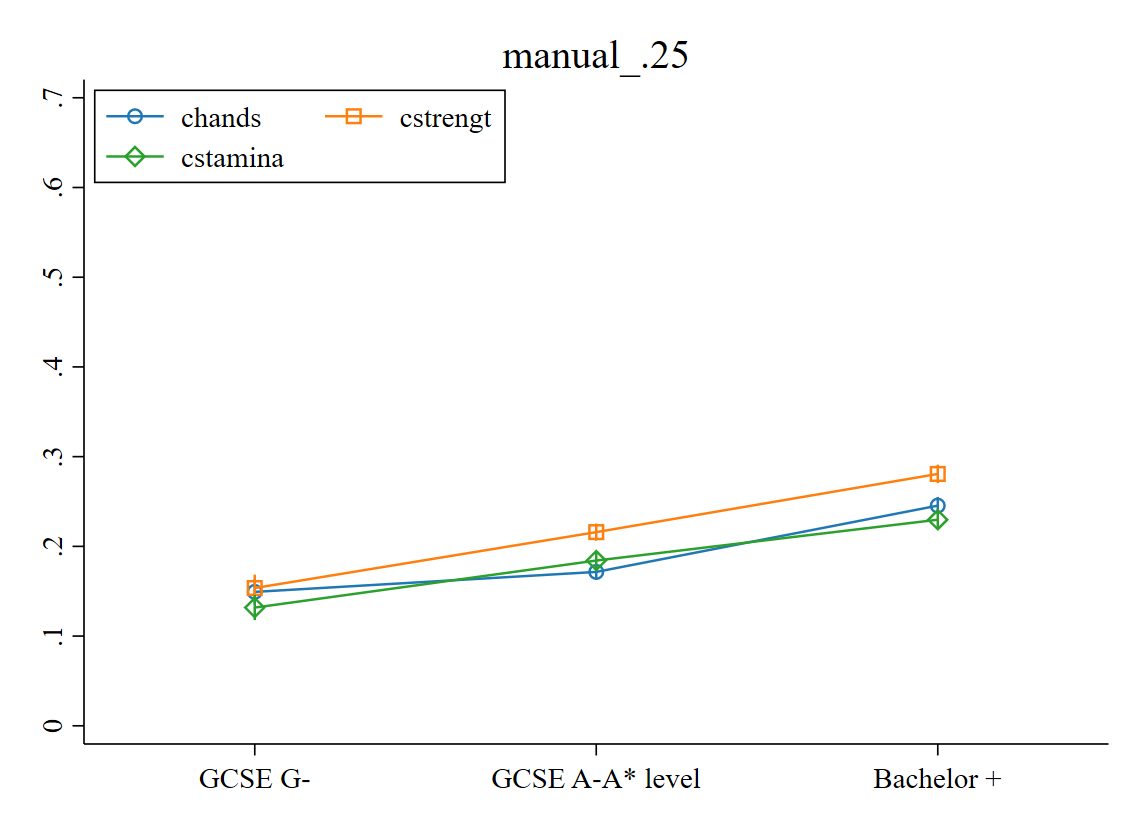
\includegraphics[width=.5\textwidth]{../results/figures//manual_25}} \subfloat[]{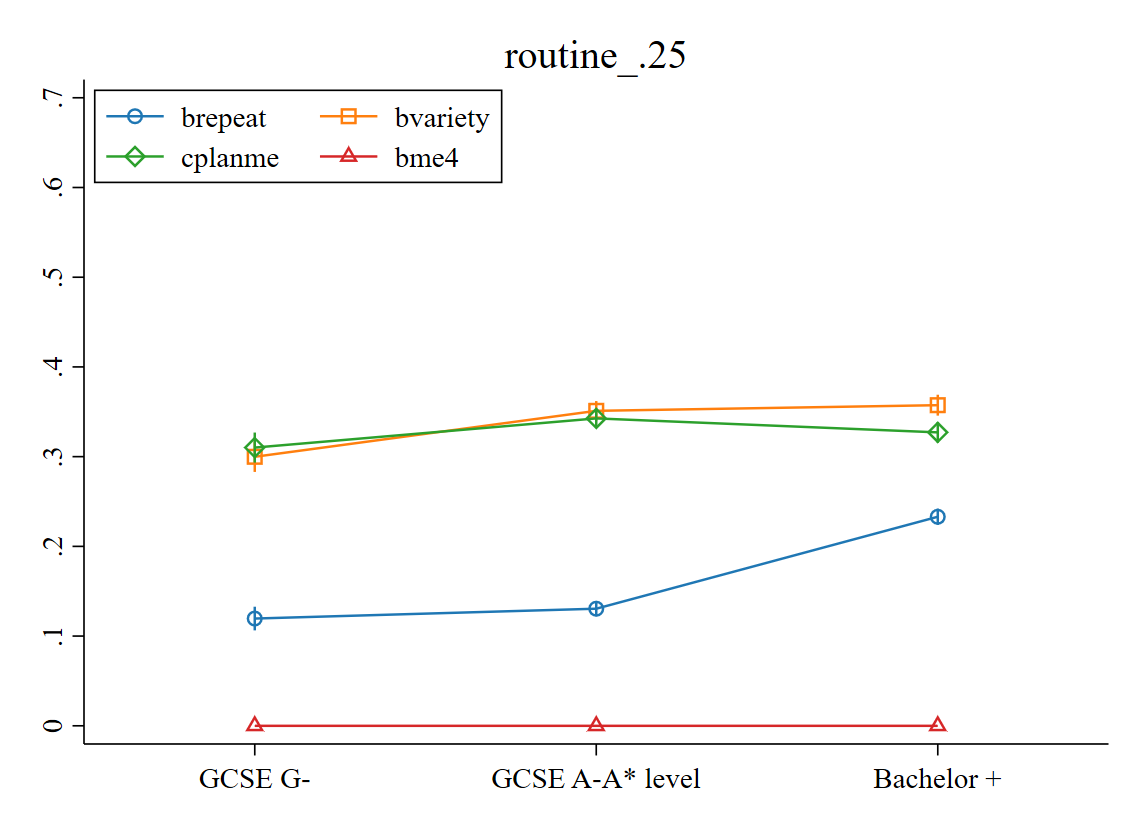
\includegraphics[width=.5\textwidth]{../results/figures//routine_25}} \\ \subfloat[]{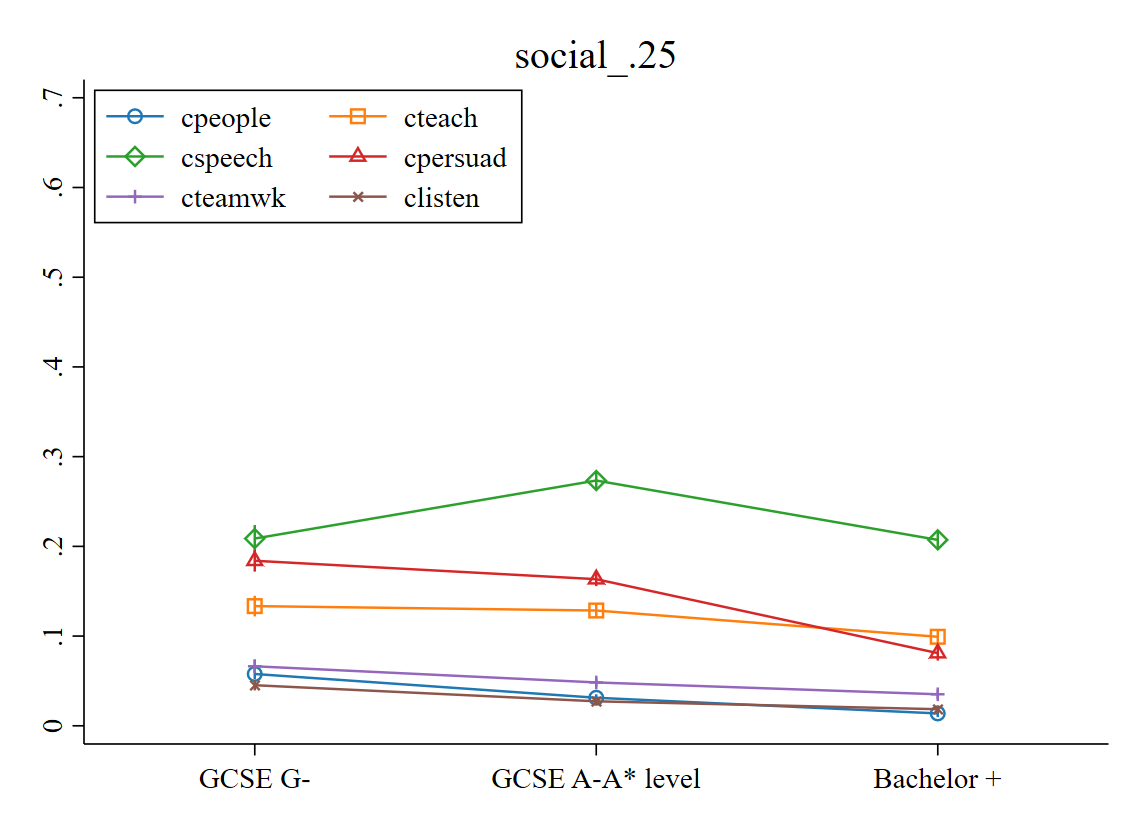
\includegraphics[width=.5\textwidth]{../results/figures//social_25}} \subfloat[]{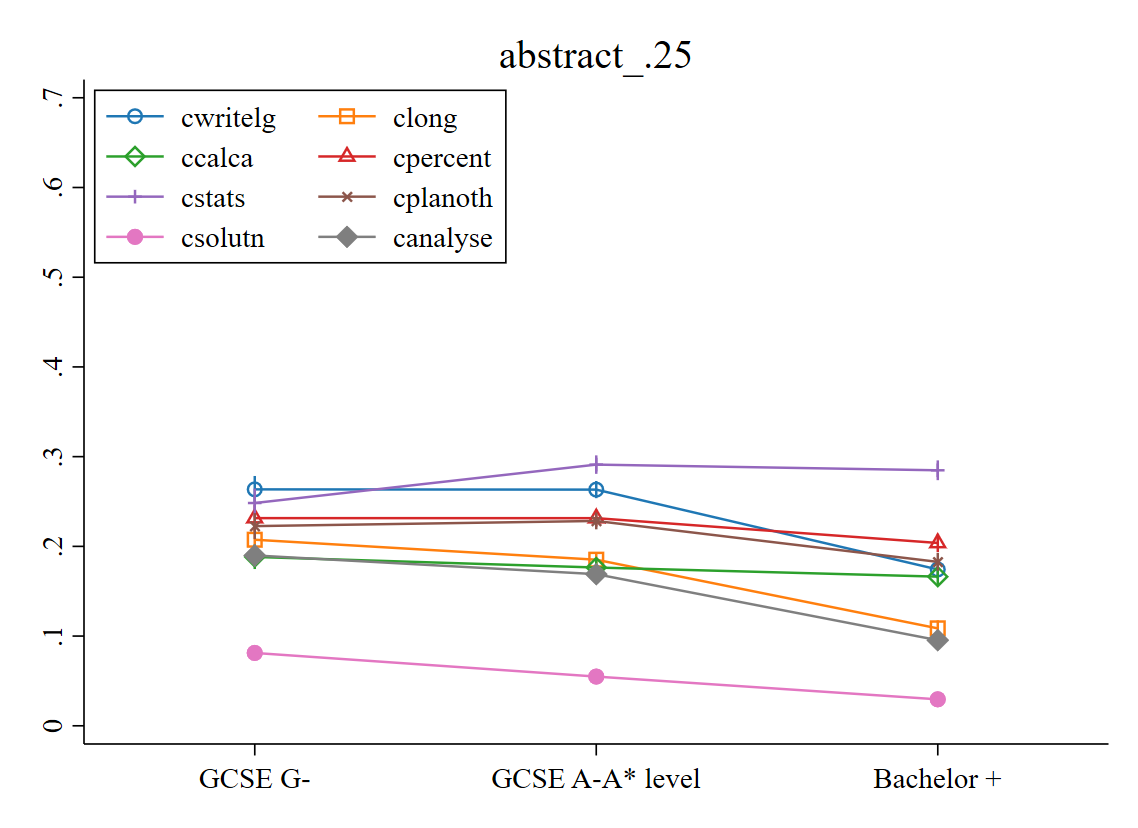
\includegraphics[width=.5\textwidth]{../results/figures//abstract_25}} \\ 
\end{figure}

%\begin{figure}[!h]
\centering
\caption{Answer 0}
\subfloat[]{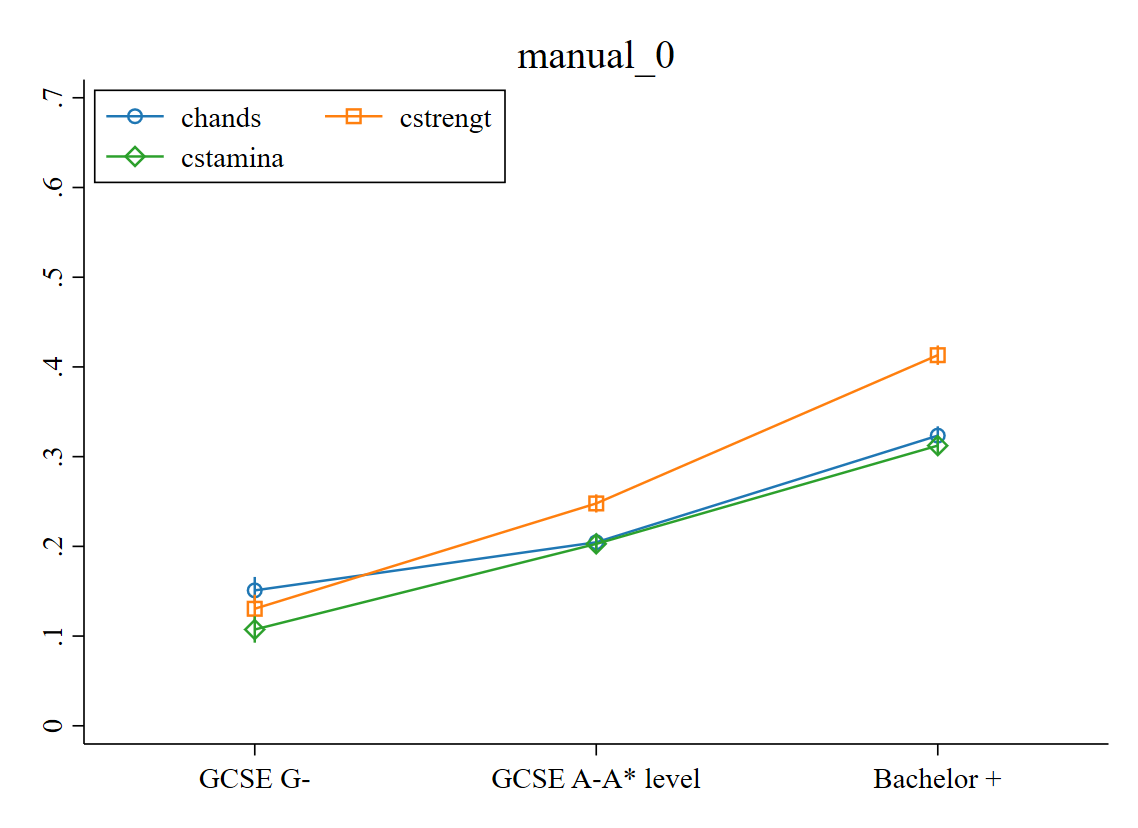
\includegraphics[width=.5\textwidth]{../results/figures//manual_0}} \subfloat[]{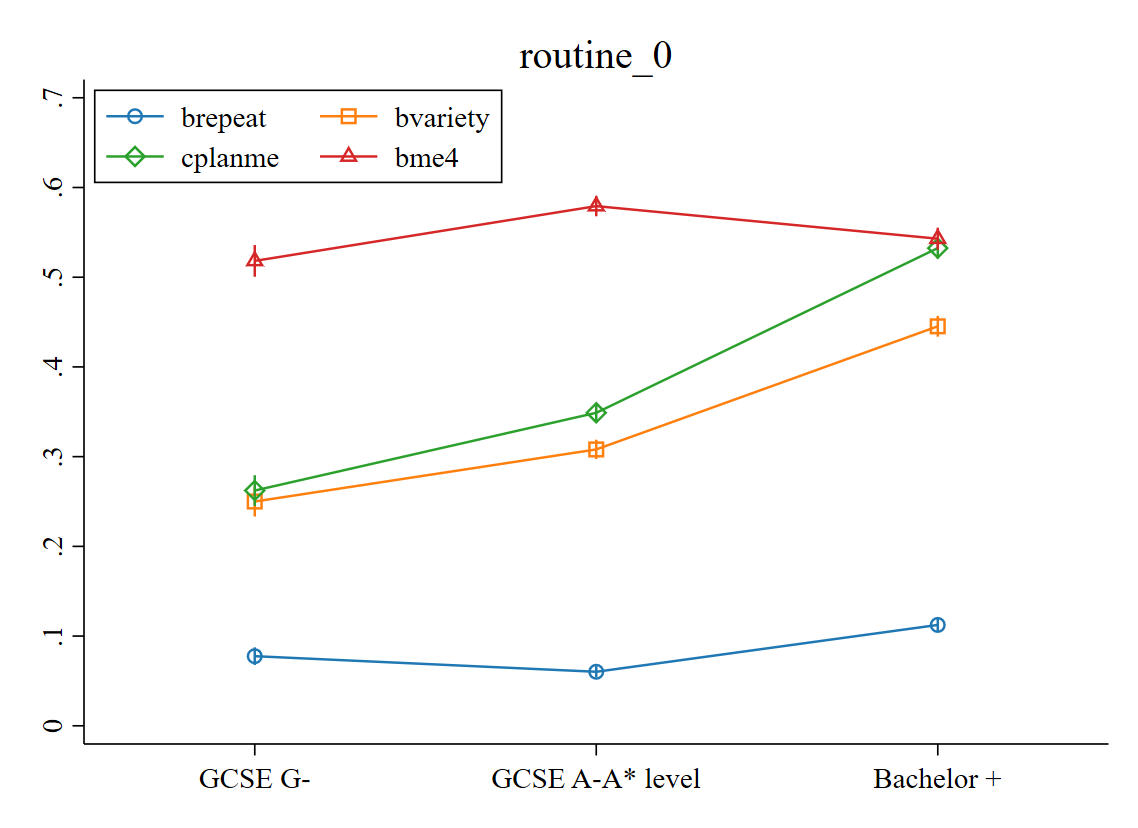
\includegraphics[width=.5\textwidth]{../results/figures//routine_0}} \\ \subfloat[]{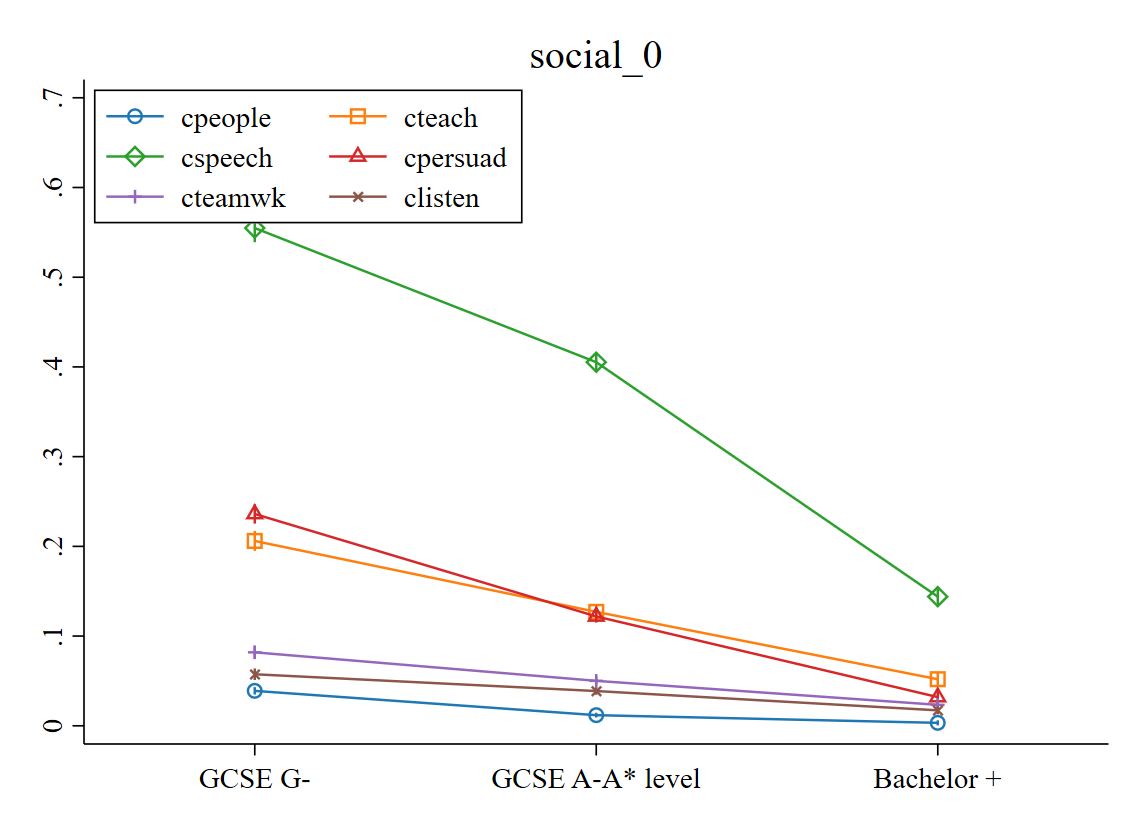
\includegraphics[width=.5\textwidth]{../results/figures//social_0}} \subfloat[]{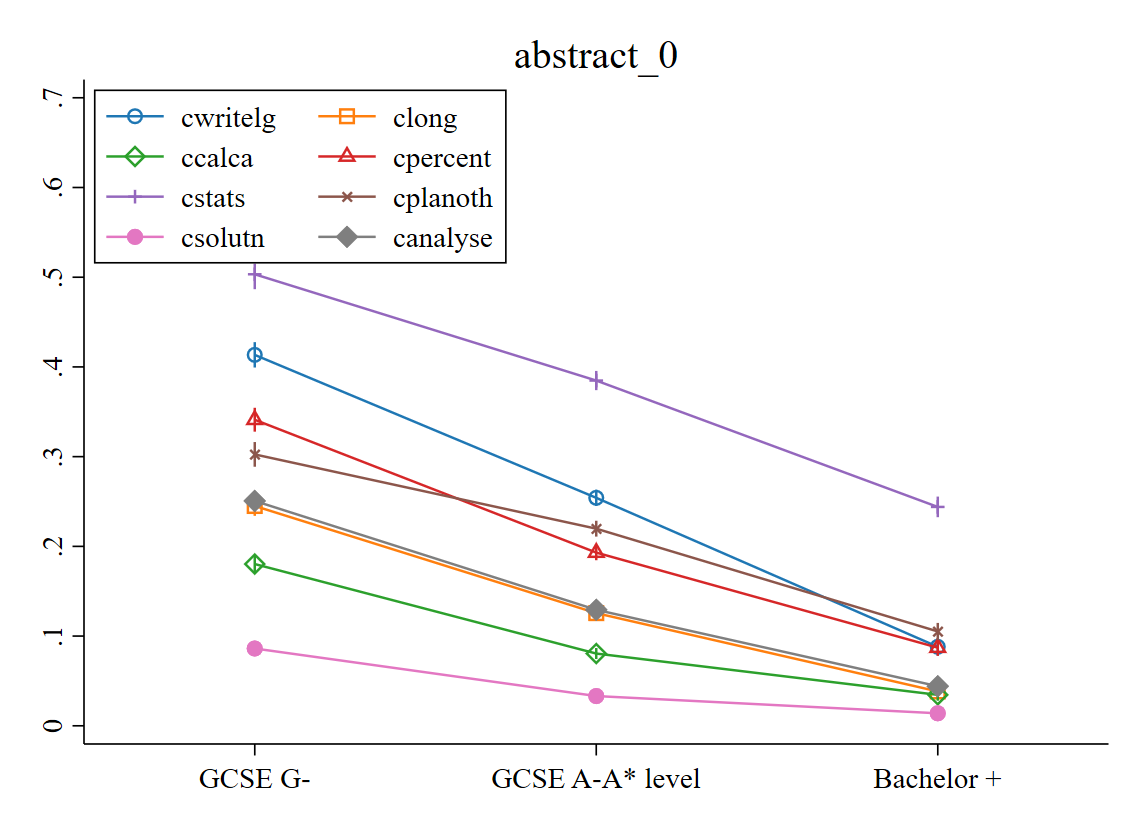
\includegraphics[width=.5\textwidth]{../results/figures//abstract_0}} \\ 
\end{figure}

%\FloatBarrier
%\section{Jobs are done differently by different education groups}
%
%We regress skill use in the job on education dummies $d_{ejt}$, and occupation fixed effects $\lambda_j$.
%\beqns
%	S_{it}=\sum_{e=1}^{3}\beta_e d_{eit}+\lambda_j+\lambda_t+\varepsilon_{it}
%\eeqns
%
%\begin{center}
\begin{threeparttable}[!h]
\caption{Within-job skill use across education groups}
\begin{tabular}{lcccc}
\toprule
\toprule
&\multicolumn{1}{c}{\textbf{Manual}}&\multicolumn{1}{c}{\textbf{Social}}&\multicolumn{1}{c}{\textbf{Adabtability}}&\multicolumn{1}{c}{\textbf{Abstract}} \\
\textbf{}&\multicolumn{1}{c}{(1)}&\multicolumn{1}{c}{(2)}&\multicolumn{1}{c}{(3)}&\multicolumn{1}{c}{(4)} \\
\midrule
HG graduates        &      -0.022\sym{***}&       0.019\sym{***}&       0.013\sym{**} &       0.029\sym{***}\\
                    &     (0.006)         &     (0.004)         &     (0.005)         &     (0.005)         \\
College+            &      -0.080\sym{***}&       0.044\sym{***}&       0.041\sym{***}&       0.063\sym{***}\\
                    &     (0.009)         &     (0.005)         &     (0.005)         &     (0.005)         \\
Baseline use        &       0.493\sym{***}&       0.647\sym{***}&       0.653\sym{***}&       0.522\sym{***}\\
                    &     (0.004)         &     (0.002)         &     (0.003)         &     (0.002)         \\
\midrule Observations&      13,515         &      13,515         &      13,515         &      13,515         \\
Occupation f.e. & \checkmark & \checkmark & \checkmark & \checkmark \\
Year f.e. & \checkmark & \checkmark & \checkmark & \checkmark \\
\bottomrule
\bottomrule
\end{tabular}
\begin{tablenotes}
\item \footnotesize \textit{Notes:} standard errors clustered at the occupation level in parenthesis. Table generated on  4 May 2023 at 10:34:18.
\end{tablenotes}
\end{threeparttable}
\end{center}

%
%
%\section{Some jobs are polarizing}
%Figure [] depicts the change in occupational employment share by education group. The yellow arrows show jobs in which the share of the \red{low education} group increased.
%
%Table \ref{tab:pol_occ} shows jobs in which the shares of employment of low and high education groups are increasing.
%
%
%Table \ref{fig:relative_use} shows low education people in the polarizing occupations used less social and more manual skills than the average occupation. Moreover, over time, the become less routine and more abstract.
%
%\begin{center}
\begin{threeparttable}[!h]
\caption{Polarizing occupations: change in occupational employment shares by education group, 2001-2017}
\label{tab:pol_occ}
\begin{tabular}{lccc}
\toprule
\toprule
&\multicolumn{1}{c}{\textbf{Low}}&\multicolumn{1}{c}{\textbf{Mid}}&\multicolumn{1}{c}{\textbf{High}} \\
\textbf{Occupation}&\multicolumn{1}{c}{(1)}&\multicolumn{1}{c}{(2)}&\multicolumn{1}{c}{(3)} \\
\midrule
2121 civil, mechanical, electrical and electronics engineers&        0.02&       -0.05&        0.03\\
2129 engineering professionals n.e.c.&        0.05&       -0.12&        0.07\\
2434 chartrd surveyors (not qntity surv)&        0.05&       -0.04&       -0.01\\
5213 Metal forming, welding and related trades&        0.07&       -0.10&        0.03\\
5312 bricklayers, masons, roofers&        0.08&       -0.14&        0.06\\
5421 printing trades&        0.08&       -0.18&        0.10\\
5431 butchers, meat cutters&        0.07&       -0.09&        0.02\\
6221 Hairdressers And Related Occupations&        0.06&       -0.15&        0.09\\
8215 Transport operatives nec&        0.06&       -0.11&        0.05\\
\bottomrule
\bottomrule
\end{tabular}
\begin{tablenotes}
\item \footnotesize \textit{Notes:} the table shows the 9 occupations (i) where the low education share increased, and (ii) survived the Benjamini-Hochberg step up procedure for the test of no change in the low education employment share at 20\% significance level. Table generated on 31 May 2023 at 10:14:01.
\end{tablenotes}
\end{threeparttable}
\end{center}

%
%\begin{figure}[!h]
\centering
\caption{Overall employment share in polarizing occupations}
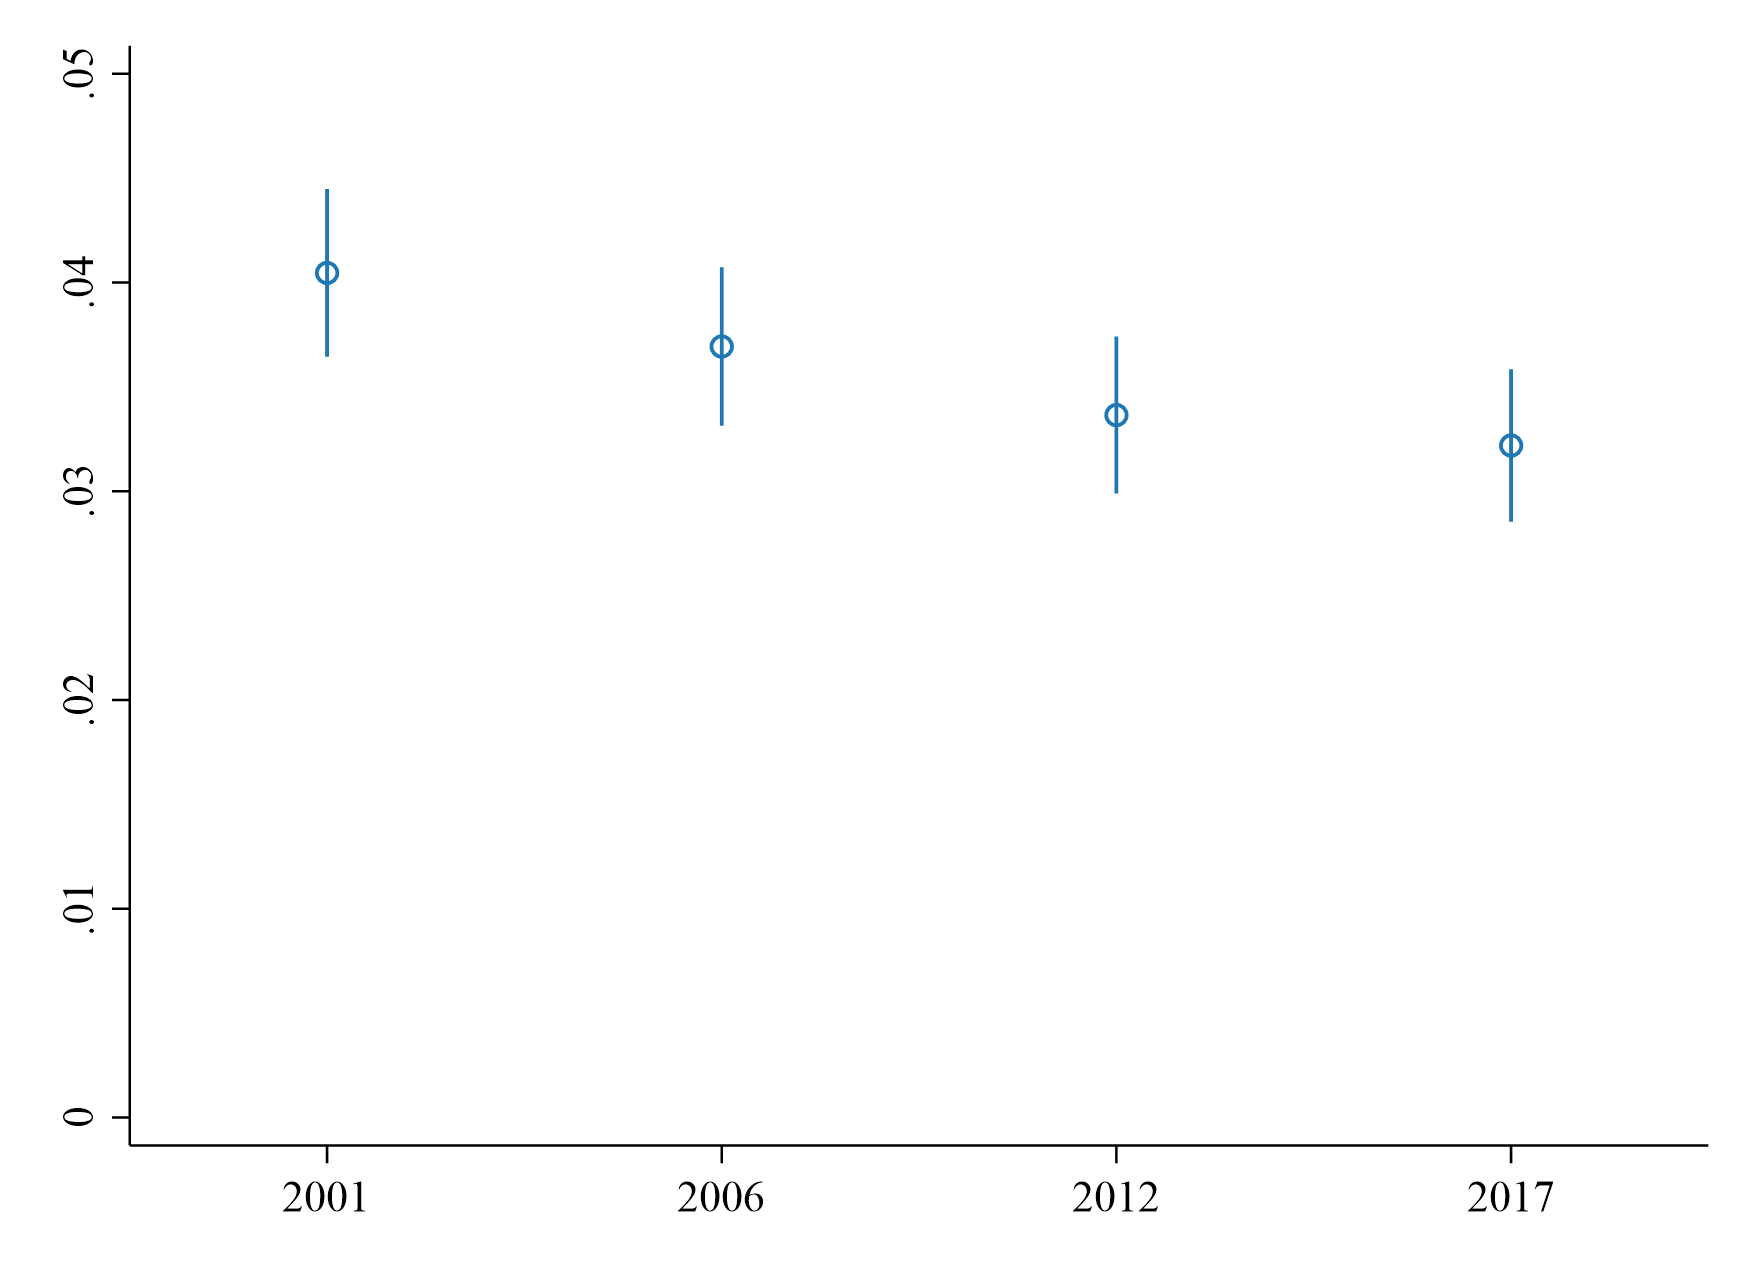
\includegraphics[width=.5\textwidth]{../results/figures//empshare_in_polarizing_occupations.png}
\par \begin{minipage}[h]{\textwidth}{\scriptsize\textbf{Note:} the figure shows the overall employment share for nine polarizing occupations Figure generated on 31 Mar 2022 at 15:16:12.}\end{minipage}
\end{figure}

%
%\begin{figure}[!h]
\centering
\caption{Relative skill use of low education individuals in polarizing occupations}
\label{fig:relative_use}
\subfloat[Skill use relative to all other occupations, 2001]{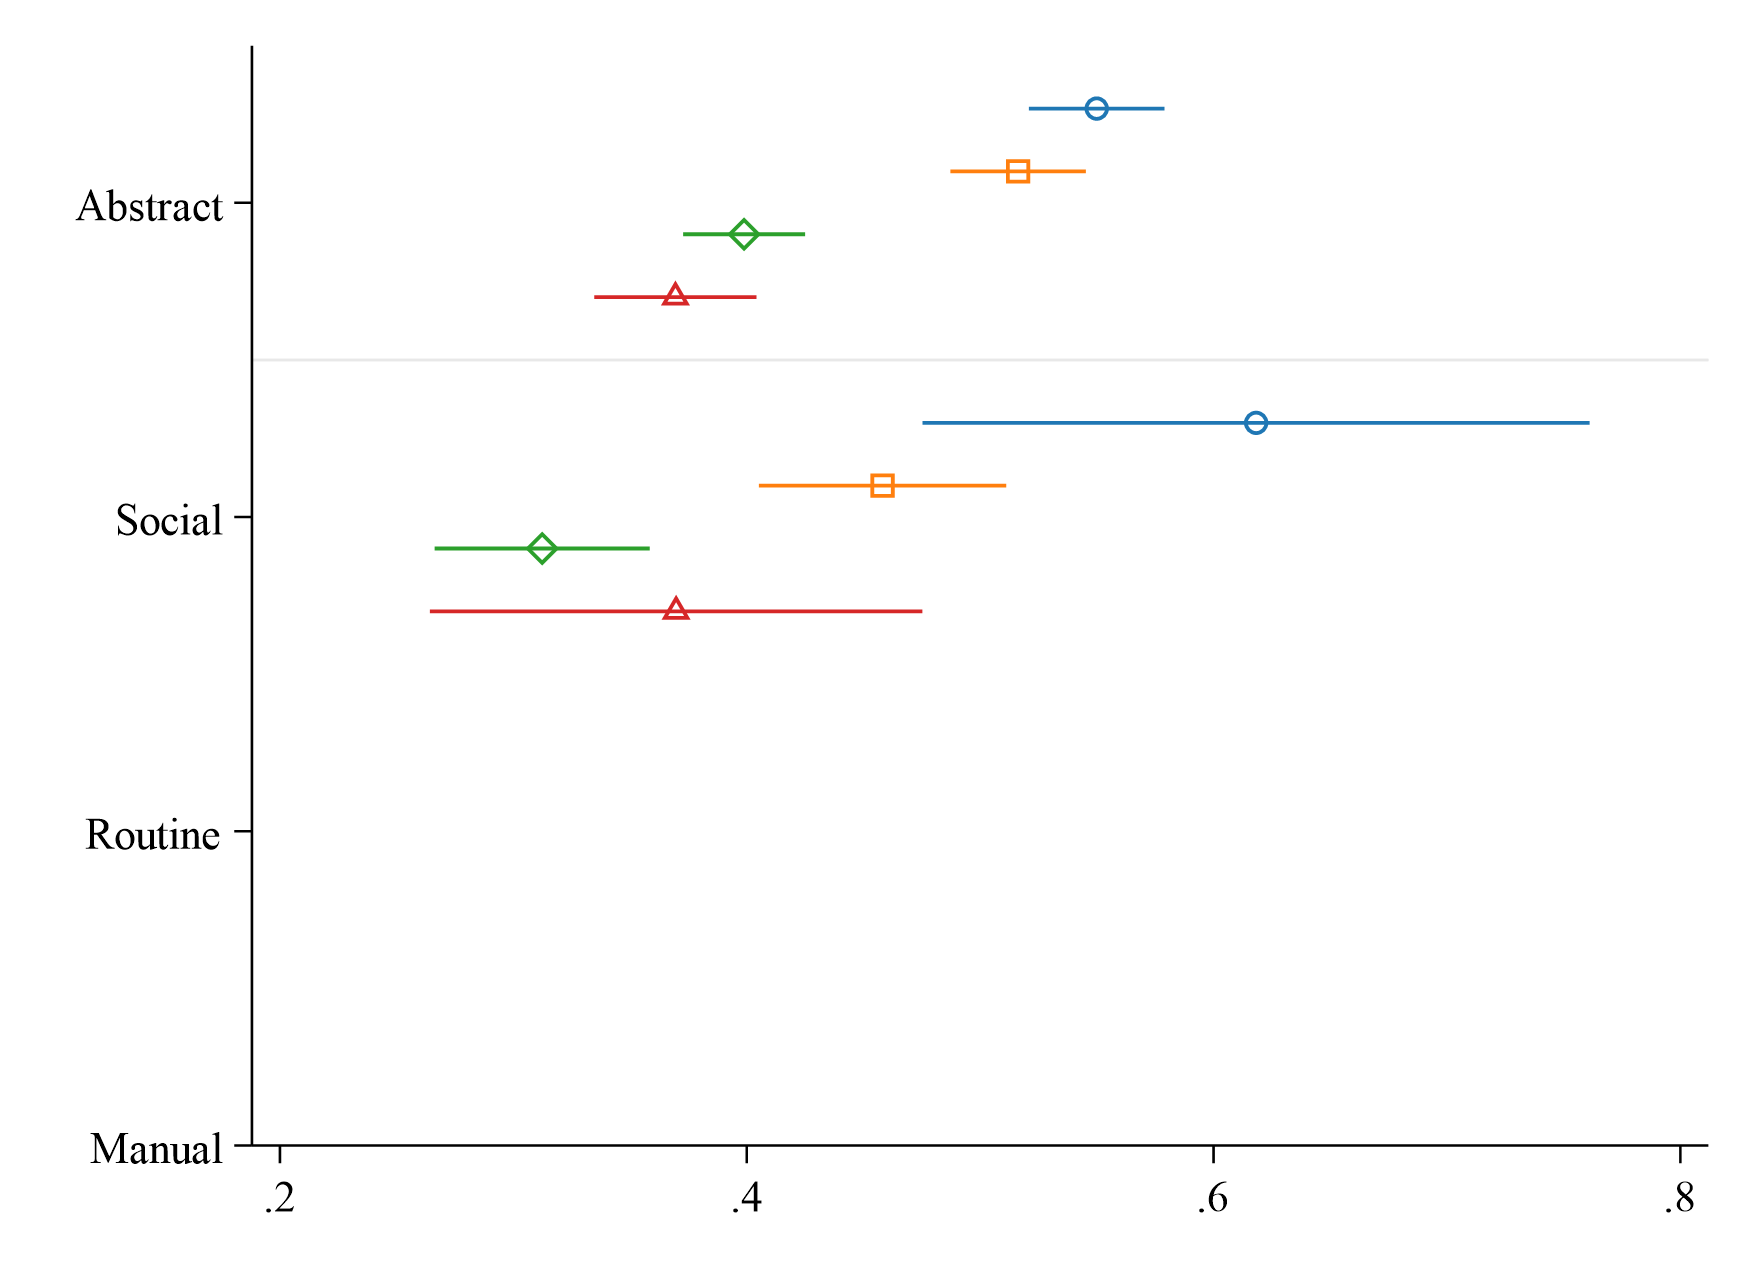
\includegraphics[width=.5\textwidth]{../results/figures//baseline_skill_use}} \subfloat[Change relative to all other occupations, 2001-2017]{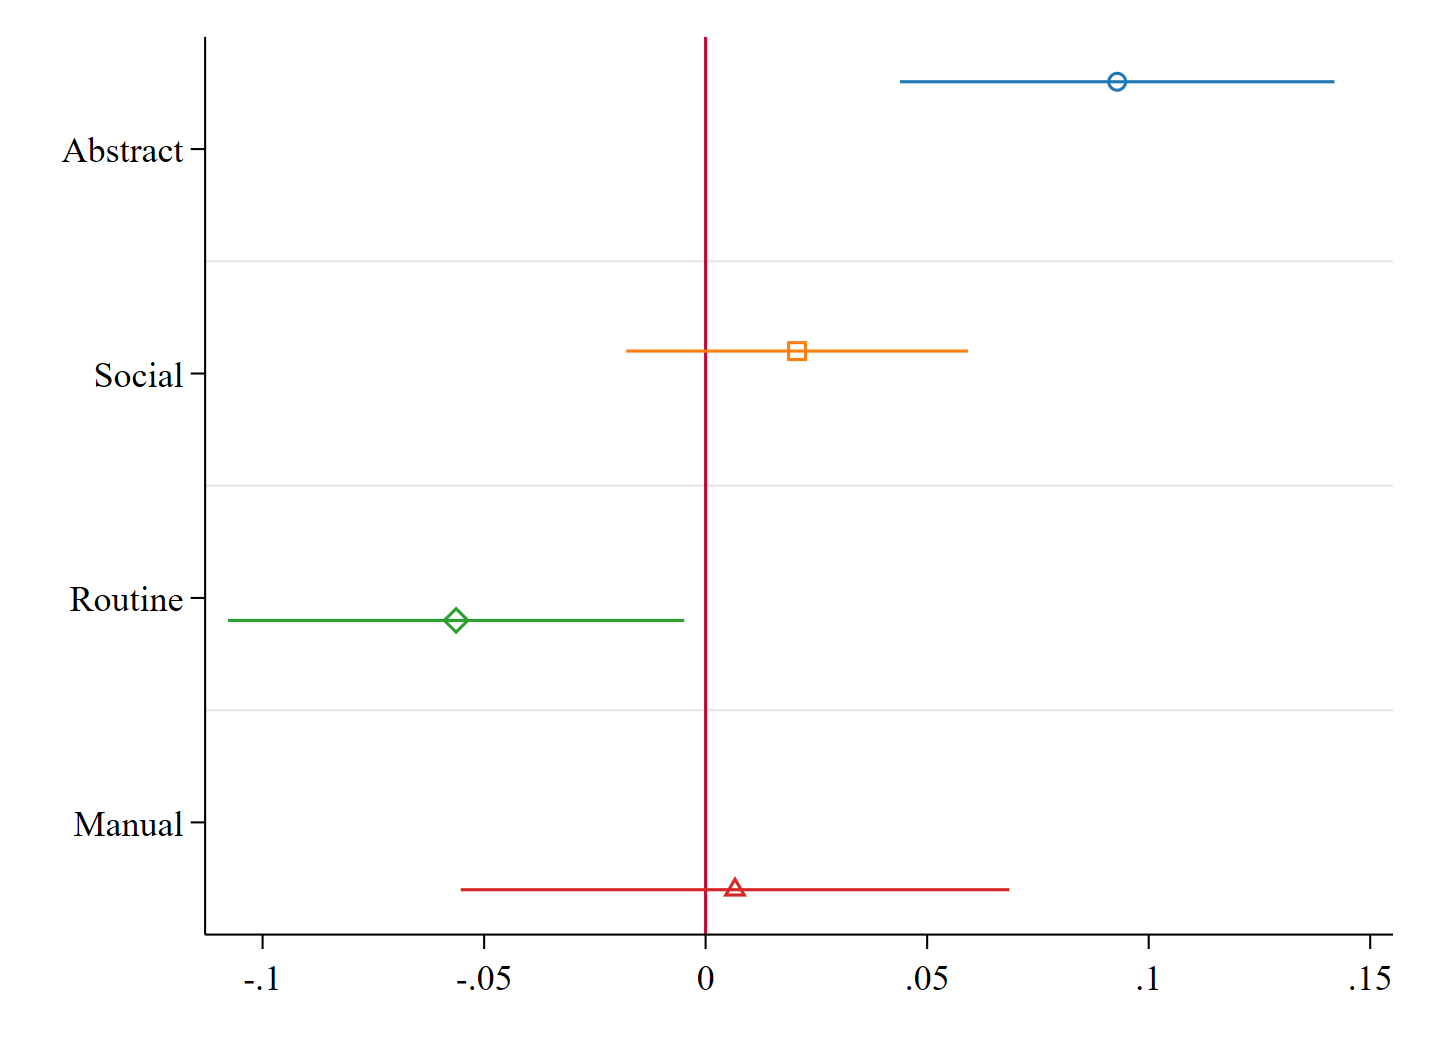
\includegraphics[width=.5\textwidth]{../results/figures//change_skill_use}} \\ 
\par \begin{minipage}[h]{\textwidth}{\scriptsize\textbf{Note:} the figure shows the relative skill use of low education individuals in polarizing occupation relative to all other occupations. The points can be roughly interpreted as percent changes relative to baseline. Figure generated on  3 May 2022 at 15:00:13.}\end{minipage}
\end{figure}

%
%\newcommand{\ntimes}{4 }
%
%\section{Estimating $\theta$}
%zLet $j$ and $e$ index occupation and education respectively. The specification is:
%\beqns
%	\Delta \ln w_{jet}=\lambda_j+\sum_{i=1}^{4}\beta_{ei}S_{iejt}+ \varepsilon_{ejt}
%\eeqns
%I get the $\theta$s computing $\theta_{ei}=\beta_{ei}/\beta_{1i}$.
%{\tiny \begin{center}
\begin{threeparttable}[!h]
\caption{$ \theta $ estimates, log average hourly pay}
\begin{tabular}{lcccccccc}
\toprule
\toprule
& \multicolumn{4}{c}{Weighted} & \multicolumn{4}{c}{Unweighted} \\
&\multicolumn{1}{c}{\textbf{Manual}}&\multicolumn{1}{c}{\textbf{Routine}}&\multicolumn{1}{c}{\textbf{Social}}&\multicolumn{1}{c}{\textbf{Abstract}}&\multicolumn{1}{c}{\textbf{Manual}}&\multicolumn{1}{c}{\textbf{Routine}}&\multicolumn{1}{c}{\textbf{Social}}&\multicolumn{1}{c}{\textbf{Abstract}} \\
\textbf{}&\multicolumn{1}{c}{(1)}&\multicolumn{1}{c}{(2)}&\multicolumn{1}{c}{(3)}&\multicolumn{1}{c}{(4)}&\multicolumn{1}{c}{(5)}&\multicolumn{1}{c}{(6)}&\multicolumn{1}{c}{(7)}&\multicolumn{1}{c}{(8)} \\
\midrule
High                &       -1.00&      -25.59&        0.50&       -0.68&       -3.72&       -4.37&        0.73&        0.92\\
                    &      (1.58)&    (293.75)&      (0.40)&      (1.84)&     (13.96)&     (16.06)&      (0.90)&      (0.66)\\
Mid                 &        1.51&       -2.48&        0.82&        1.28&        0.08&       -0.84&        0.18&        0.26\\
                    &      (0.88)&     (35.32)&      (0.34)&      (1.38)&      (2.51)&      (4.85)&      (0.74)&      (0.42)\\
Observations        &         396&         396&         396&         396&         396&         396&         396&         396\\
\bottomrule
\bottomrule
\end{tabular}
\begin{tablenotes}
\item \footnotesize \textit{Notes:} Robust standard errors in parenthesis. Columns 1 to 4 weighted by LFS-cell size. Table generated on 20 Mar 2022 at 19:03:26.
\end{tablenotes}
\end{threeparttable}
\end{center}
}
%{\tiny \begin{center}
\begin{threeparttable}[!h]
\caption{$ \theta $ estimates, log average weekly pay}
\begin{tabular}{lcccccccc}
\toprule
\toprule
& \multicolumn{4}{c}{Weighted} & \multicolumn{4}{c}{Unweighted} \\
&\multicolumn{1}{c}{\textbf{Manual}}&\multicolumn{1}{c}{\textbf{Routine}}&\multicolumn{1}{c}{\textbf{Social}}&\multicolumn{1}{c}{\textbf{Abstract}}&\multicolumn{1}{c}{\textbf{Manual}}&\multicolumn{1}{c}{\textbf{Routine}}&\multicolumn{1}{c}{\textbf{Social}}&\multicolumn{1}{c}{\textbf{Abstract}} \\
\textbf{}&\multicolumn{1}{c}{(1)}&\multicolumn{1}{c}{(2)}&\multicolumn{1}{c}{(3)}&\multicolumn{1}{c}{(4)}&\multicolumn{1}{c}{(5)}&\multicolumn{1}{c}{(6)}&\multicolumn{1}{c}{(7)}&\multicolumn{1}{c}{(8)} \\
\midrule
High                &       -0.35&       33.68&        0.31&       -0.56&       -0.31&       -2.84&        0.14&        8.32\\
                    &      (1.11)&    (483.22)&      (0.31)&      (0.92)&      (0.80)&      (3.50)&      (0.91)&    (101.61)\\
Mid                 &        1.37&        0.47&        0.65&        0.59&        0.57&       -0.69&        0.83&       -2.19\\
                    &      (0.77)&     (11.80)&      (0.25)&      (0.51)&      (0.56)&      (1.33)&      (1.21)&     (29.31)\\
Observations        &         396&         396&         396&         396&         396&         396&         396&         396\\
\bottomrule
\bottomrule
\end{tabular}
\begin{tablenotes}
\item \footnotesize \textit{Notes:} Robust standard errors in parenthesis. Columns 1 to 4 weighted by LFS-cell size. Table generated on 20 Mar 2022 at 19:03:26.
\end{tablenotes}
\end{threeparttable}
\end{center}
}
%
%\href{https://www.dropbox.com/s/dnt84rs90zac1h9/t_stats.txt?dl=0}{Occupations with increasing low share}
%
%\begin{center}
\begin{threeparttable}[!h]
\caption{Skill use in occupations with increased low share}
\begin{tabular}{lcc}
\toprule
\toprule
\textbf{}&\multicolumn{1}{c}{\textbf{2001}}&\multicolumn{1}{c}{\textbf{2017}} \\
\midrule
\textbf{abstract} \\
All other           &        2.69&        2.77\\
                    &      (0.07)&      (0.08)\\
Increased low share &        2.77&        3.25\\
                    &      (0.11)&      (0.03)\\
Difference          &        0.08&        0.48\\
                    &      (0.13)&      (0.09)\\
\textbf{social} \\
All other           &        3.32&        3.38\\
                    &      (0.06)&      (0.07)\\
Increased low share &        3.09&        3.24\\
                    &      (0.05)&      (0.05)\\
Difference          &       -0.23&       -0.14\\
                    &      (0.07)&      (0.08)\\
\textbf{routine} \\
All other           &        2.51&        2.65\\
                    &      (0.04)&      (0.05)\\
Increased low share &        2.35&        2.24\\
                    &      (0.12)&      (0.06)\\
Difference          &       -0.16&       -0.41\\
                    &      (0.13)&      (0.08)\\
\textbf{manual} \\
All other           &        3.12&        3.28\\
                    &      (0.08)&      (0.09)\\
Increased low share &        4.01&        4.20\\
                    &      (0.21)&      (0.13)\\
Difference          &        0.89&        0.92\\
                    &      (0.23)&      (0.15)\\
\bottomrule
\bottomrule
\end{tabular}
\end{threeparttable}
\end{center}

%\begin{center}
\begin{threeparttable}[!h]
\caption{Employment share of deskilling occupations by year}
\begin{tabular}{lcc}
\toprule
\toprule
\textbf{}&\multicolumn{1}{c}{\textbf{Employment share}}&\multicolumn{1}{c}{\textbf{ }} \\
\midrule
year=2001           &       0.039\\
                    &     (0.002)\\
year=2006           &       0.039\\
                    &     (0.002)\\
year=2012           &       0.037\\
                    &     (0.002)\\
year=2017           &       0.035\\
                    &     (0.002)\\
Observations        &       37535\\
\bottomrule
\bottomrule
\end{tabular}
\end{threeparttable}
\end{center}

%\begin{center}
\begin{threeparttable}[!h]
\caption{Education employment share of deskilling occupations by year}
\begin{tabular}{lccc}
\toprule
\toprule
\textbf{}&\multicolumn{1}{c}{\textbf{Low}}&\multicolumn{1}{c}{\textbf{Mid}}&\multicolumn{1}{c}{\textbf{High}} \\
\midrule
year=2001           &       0.180&       0.723&       0.097\\
                    &     (0.019)&     (0.024)&     (0.018)\\
year=2006           &       0.184&       0.707&       0.109\\
                    &     (0.019)&     (0.023)&     (0.017)\\
year=2012           &       0.156&       0.685&       0.158\\
                    &     (0.020)&     (0.024)&     (0.018)\\
year=2017           &       0.145&       0.663&       0.192\\
                    &     (0.019)&     (0.024)&     (0.018)\\
Observations        &        1503&        1503&        1503\\
\bottomrule
\bottomrule
\end{tabular}
\end{threeparttable}
\end{center}

%\begin{center}
\begin{threeparttable}[!h]
\caption{Education employment share of deskilling occupations by year, includes occ fe}
\begin{tabular}{lccc}
\toprule
\toprule
\textbf{}&\multicolumn{1}{c}{\textbf{Low}}&\multicolumn{1}{c}{\textbf{Mid}}&\multicolumn{1}{c}{\textbf{High}} \\
\midrule
year=2001           &       0.000&       0.000&       0.000\\
                    &         (.)&         (.)&         (.)\\
year=2006           &       0.002&      -0.015&       0.014\\
                    &     (0.026)&     (0.033)&     (0.024)\\
year=2012           &      -0.022&      -0.037&       0.060\\
                    &     (0.027)&     (0.034)&     (0.025)\\
year=2017           &      -0.033&      -0.055&       0.088\\
                    &     (0.027)&     (0.033)&     (0.025)\\
Observations        &        1503&        1503&        1503\\
\bottomrule
\bottomrule
\end{tabular}
\end{threeparttable}
\end{center}

%
%
%\begin{figure}
%	\caption{Change in employment shares: 2001-2017}
%	\addfig{1}{../results/figures/direction_triangle}
%\end{figure}
%
%\FloatBarrier
%\href{https://www.dropbox.com/s/pxkgmtnkhq6c0j1/deskilling_occupations.txt?dl=0}{Occupations in yellow}
%\begin{figure}
%\caption{Abstract, Routine and Manual}
%\subfloat[Low-mid]{\animategraphics[loop,controls,width=\linewidth]{1}{../results/figures/border_triangle_mra12_}{2001}{2017}}
%\end{figure}
%\begin{figure}
%\ContinuedFloat
%\subfloat[Low-High]{\animategraphics[loop,controls,width=\linewidth]{1}{../results/figures/border_triangle_mra13_}{2001}{2017}}
%\end{figure}
%\begin{figure}
%\ContinuedFloat
%\subfloat[Mid-High]{\animategraphics[loop,controls,width=\linewidth]{1}{../results/figures/border_triangle_mra23_}{2001}{2017}}
%\end{figure}
%
%\begin{figure}
%	\caption{Social, Routine and Manual}
%	\subfloat[Low-mid]{\animategraphics[loop,controls,width=\linewidth]{1}{../results/figures/border_triangle_mrs12_}{2001}{2017}}
%\end{figure}
%\begin{figure}
%	\ContinuedFloat
%	\subfloat[Low-High]{\animategraphics[loop,controls,width=\linewidth]{1}{../results/figures/border_triangle_mrs13_}{2001}{2017}}
%\end{figure}
%\begin{figure}
%	\ContinuedFloat
%	\subfloat[Mid-High]{\animategraphics[loop,controls,width=\linewidth]{1}{../results/figures/border_triangle_mrs23_}{2001}{2017}}
%\end{figure}
%
%
%\begin{figure}
%	\caption{Abstract, Routine and Social}
%	\subfloat[Low-mid]{\animategraphics[loop,controls,width=\linewidth]{1}{../results/figures/border_triangle_sra12_}{2001}{2017}}
%\end{figure}
%\begin{figure}
%	\ContinuedFloat
%	\subfloat[Low-High]{\animategraphics[loop,controls,width=\linewidth]{1}{../results/figures/border_triangle_sra13_}{2001}{2017}}
%\end{figure}
%\begin{figure}
%	\ContinuedFloat
%	\subfloat[Mid-High]{\animategraphics[loop,controls,width=\linewidth]{1}{../results/figures/border_triangle_sra23_}{2001}{2017}}
%\end{figure}
%
%
%\begin{figure}
%	\caption{Abstract, Social and Manual}
%	\subfloat[Low-mid]{\animategraphics[loop,controls,width=\linewidth]{1}{../results/figures/border_triangle_msa12_}{2001}{2017}}
%\end{figure}
%\begin{figure}
%	\ContinuedFloat
%	\subfloat[Low-High]{\animategraphics[loop,controls,width=\linewidth]{1}{../results/figures/border_triangle_msa13_}{2001}{2017}}
%\end{figure}
%\begin{figure}
%	\ContinuedFloat
%	\subfloat[Mid-High]{\animategraphics[loop,controls,width=\linewidth]{1}{../results/figures/border_triangle_msa23_}{2001}{2017}}
%\end{figure}
%
%\FloatBarrier
%
%\section{Estimating $\theta$}
%\label{sec:model}
%%Fix the notation here
%We use two key equations from the model:
%\beqn
%\sum_{i=1}^I\theta_i^eS_{i}^e(J)&=&1 \\
%d\ln f^e(J)&=&\frac{\varepsilon}{1-\varepsilon}\sum_i\theta_i^e(d\ln A_i - K^e)S_i^e(J) \label{eq:empshare}
%\eeqn
%where $e\in\{1,2,3\}$ indexes the education group and $i$ indexes the skill. We impose several normalizations to the model:
%\bitem 
%\item Skill acquisition costs are 1 for the low education group $\theta_i^1=1$.
%\item Manual acquisition costs are 1 for all education groups $\theta_1^e=1$.
%\eitem
%
%
%We do not observe the skill indexes $S_{i}^e(J)$. We estimate them using information from 22 questions from the SES survey. These questions typically ask respondents to rate how important a given task or job trait is for their job. These ratings go from 1 to 5, 5 being very important. We combine all these answers into an index as follows:
%\beqn
%S_{i}(J)=\sum_{j=1}^{||i||}\alpha_{ij}\sum_{l=1}^5c_{ijl}1_{d_{ij}=l}
%\eeqn
%where $d_{jm}\in\{1,2,3,4,5\}$ is the individual's answer to the SES question $ij$. I abused notation  by indicating the number of SES questions in index $i$ with $||i||$.  $\alpha_{ij}$ and $c_{ijl}$ are parameters to estimate. The scales $c_{ijl}$  are the numeric values we give to each answer in the Likert scale. The $\alpha_{ij}$ are weights we give to each question within the index. For all questions we normalize the lowest scale value to zero ($c_{ij1}=0, \forall i,j$) and highest value to 1 ($c_{ij5}=0,\forall i,j$). The only restriction on the weights  $\alpha_{ij}$ is that they must be non-negative.
%
%\subsection{Data I use for estimation}
%The data I feed to the algorithm satisfies two restrictions:
%\benu
%	\item I restrict to jobs that I observe as \red{\textbf{core}} in any two consecutive SES years.
%	\item As of now, I \red{\textbf{am not}} applying any restriction by education group. 
%	
%	So, for example I am including observations of low education individuals that are in high-education core jobs.
%\eenu
%
%\subsection{Procedure}
%
%We start by guessing values for the weights $\alpha_{jm}$ and the Likert scales $c_{jml}$. This gives us an initial guess for the skill indexes $S_{\theta,m}(J)$.
%
%\paragraph{Step 1: estimate skill acquisition costs:} given the guess for $S_{\theta,m}(J)$ we estimate the skill acquisition costs $\theta_{i}^e$ using the empirical analogous of equation \eqref{eq:empshare}.
%\beqns
%d\ln f^e(J)&=&\sum_i\beta_i^eS_i^e(J) + \lambda_I+v^e(J)
%\eeqns
%In this equation we constrain the $\theta_{i}$ to be positive by estimating the following non-linear equation:
%\beqns
%d\ln f^1(J)&=&\sum_i\beta_i^1S_i^e(J) + v^1(J)\\
%d\ln f^e(J)&=&\beta_1^eS_1^e(J)+\sum_{i=2}^4(\sqrt{\theta_i^e})^2\left(\beta_{i}^1-\beta_{1}^1+\beta_{1}^e\right)S_i^e(J) + v^e(J), e>1\\
%\eeqns
%%We can compute the skill acquisition costs out of the $\beta_i^e$ using:
%\beqn
%\theta_i^e=\frac{\beta_i^e}{\beta_i^1-\beta_1^1+\beta_1^e} \label{eq:empirical}
%\eeqn
%
%\paragraph{Step 2: estimate Likert scales and question weights} we use the $\theta_i^e$ estimated in the step above to compute the Likert scales and the question weights. We choose scales and weights to minimize the MSE from equation \eqref{eq:skill_sum}: 
%
%\beqns
%\min_{\alpha_{jm},c_{jml}}\frac{1}{N}\left[\sum_{m=1}^I\theta_j^eS_{m}^e-1\right]^2 \text{ s.t. }  S_{m}^e=\sum_{j=1}^{||m||}\alpha_{jm}\sum_{l=1}^5c_{jml}1_{d_{ijm}=l}
%\eeqns
%
%\paragraph{Iterate until $\theta$ converges}: we iterate this procedure until the skill acquisition costs converge: 
%\beqns
%||\Theta_n-\Theta_{n-1}||<0.01
%\eeqns
%
%where $\Theta_n$ is the vector of skill acquisition costs estimated in step $n$\footnote{You could argue that 0.01 is a loose tolerance threshold is large, but I was getting bored of having the code running. I just wanted to see a likely convergence point.}.
%
%\section{$\theta$s from regressions out of simple average skill indexes}
%Here I show estimated skill acquisition costs when I compute them using simple average indexes. These $\theta_i$ come from the regression:
%\beqn
%d\ln f^e(J)&=&\sum_i\beta_i^eS_i^e(J)\\
%\eeqn
%where:
%\beqns
%\beta_{i}^e=\frac{\varepsilon}{1-\varepsilon}\theta_i^e(d\ln A_i - K^e)
%\eeqns
%I define the indexes as follows:
%\beqns
%S_i(J)&=&\frac{\tilde{S}_i(J)}{\sum_k^K\tilde{S}_k(J) } \\
%\eeqns
%where $S_k(J)$ is the simple average of the scores I assigned to each SES question:
%\beqns
%S_{i}(J)=\frac{1}{||i||}\sum_{j=1}^{||i||}\sum_{l=1}^5c_{ijl}1_{d_{ij}=l}\\
%\eeqns
%remember that the SES questions have possible answer going from 1 to 5. I normalized these answers $c_{ijl}$  to be between zero and one.
%\beqns
%c_{ijl}=\frac{l-1}{4}
%\eeqns
%\subsection{Results}
%Weighted result weights observation by the occupation-years cells size. The implied thetas are in these files:
%\bitem
%\item Unweighted $\theta$s: \href{https://www.dropbox.com/s/epmal84fzmnwiam/unweighted_thetas.txt?dl=0}{click here}
%\item Weighted $\theta$s: \href{https://www.dropbox.com/s/bkq8o6zcjmgpjf8/weighted_thetas.txt?dl=0}{click here}
%\eitem
%\FloatBarrier
%\begin{center}
\begin{threeparttable}[!h]
\caption{Estimates of $\beta_{i}^e$}
\begin{tabular}{lcc}
\toprule
\toprule
&\multicolumn{1}{c}{\textbf{Unweighted}}&\multicolumn{1}{c}{\textbf{Weighted}} \\
\textbf{}&\multicolumn{1}{c}{(1)}&\multicolumn{1}{c}{(2)} \\
\midrule
manual1             &        0.03&        0.03\\
                    &      (0.11)&      (0.11)\\
abstract1           &       -0.69&       -0.69\\
                    &      (0.26)&      (0.26)\\
social1             &       -0.01&       -0.01\\
                    &      (0.29)&      (0.29)\\
routine1            &       -0.19&       -0.19\\
                    &      (0.18)&      (0.18)\\
manual2             &        0.58&        0.58\\
                    &      (0.28)&      (0.28)\\
abstract2           &       -2.78&       -2.78\\
                    &      (0.60)&      (0.60)\\
social2             &        2.31&        2.31\\
                    &      (0.66)&      (0.66)\\
routine2            &        0.56&        0.56\\
                    &      (0.37)&      (0.37)\\
manual3             &        0.06&        0.06\\
                    &      (0.13)&      (0.13)\\
abstract3           &        0.17&        0.17\\
                    &      (0.15)&      (0.15)\\
social3             &       -0.11&       -0.11\\
                    &      (0.18)&      (0.18)\\
routine3            &       -0.62&       -0.62\\
                    &      (0.24)&      (0.24)\\
n\_occupations       &            &            \\
N                   &       4,687&       4,687\\
r2                  &        0.07&        0.07\\
\bottomrule
\bottomrule
\end{tabular}
\begin{tablenotes}
\item \footnotesize \textit{Notes:} Standard errors clustered at the occupation level. Estimates include industry by education fixed-effects. Table generated on  8 Mar 2022 at 16:33:20.
\end{tablenotes}
\end{threeparttable}
\end{center}

%\begin{table}[htbp]\centering \caption{$\theta_{ie}$ estimates} \begin{tabular}{l*{4}{c}} \toprule
            &      manual&     routine&      social&    abstract\\
\midrule
Low         &        0.46&        0.40&        0.37&        0.64\\
Mid         &        0.65&        0.29&        0.20&        0.67\\
High        &        0.59&        0.45&        0.25&        0.61\\
\bottomrule
\end{tabular}
\end{table}

%\FloatBarrier
%%
%%\section{Simulating data}
%%I simulate data based on equations:
%%\beqn
%%\sum_{i=1}^I\theta_i^eS_{i}^e(J)&=&1 \label{eq:skill_sum}\\
%%d\ln f^e(J)&=&\frac{\varepsilon}{1-\varepsilon}\sum_i\theta_i^e(d\ln A_i - K^e)S_i^e(J) \label{eq:empshares}
%%\eeqn
%%\subsection{Procedure}
%%\subsubsection{Assumptions}
%%I assume a world of 2 education groups, 2 skills, and each skill is made up of a unique dummy variable:
%%\newline
%%
%%\noindent\textbf{Model parameters:}
%%\bitem 
%%	\item $\varepsilon=0.5$
%%	\item $d\ln A=\begin{pmatrix}
%%		3 & -2 \\
%%		3 & -2
%%	\end{pmatrix}$
%%	\item $K^e=2$
%%	\item $\theta=\begin{pmatrix}
%%		1 & 1 \\
%%		1 & 0.5
%%	\end{pmatrix}$
%%\eitem 
%%In this world equations equation \eqref{eq:skill_sum} holds at the job level\footnote{It makes a difference whether I assume this is true at the job level, or at the individual level!} with some noise so that:
%%\beqns
%%	S_1^e(J)=1-\theta_2^eS_2^e(J)+\nu(J) \label{eq:sim_prob}
%%\eeqns
%%because the skills are dummy variables, then $S_i^e(J)$ is simply the probability that the skill variable is equal to 1 for job $J$ and education $e$. Given $S_2^e(J)$ and $\nu(J)$, equation \eqref{eq:sim_prob} defines the probabilities to generate data for skill 1. Throughout I assume $p_2^1(J)=\frac{1}{8}$, $p_2^2(J)=\frac{7}{8}$ and $v(J) \sim U[  -m,m ]$. I chose $m$ so that the probabilities are well defined.
%%
%%Next, I generate employment share data using: 
%%\beqns
%%d\ln f^e(J)&=&\frac{\varepsilon}{1-\varepsilon}\sum_i\theta_i^e(d\ln A_i - K^e)S_i^e(J)+\kappa(J)
%%\eeqns
%%where $\kappa(J)\sim N(0,1)$.
%%
%%\paragraph{Estimated $\theta$}
%%\bitem 
%%\item $\theta=\begin{pmatrix}
%%	1 & 1 \\
%%	1 & 0.53
%%\end{pmatrix}$
%%\eitem 
%
%
%%
%%\red{Put this in a proof later}
%%The normalization on the manual index implies:
%%\beqns
%%\beta_i^1=d\ln A_i-K^e
%%\eeqns
%%therefore:
%%\beqns
%%d\ln A_1&=&\beta_1^1+K\\
%%K^e&=&-\beta_1^e+\beta_1^1+K^e
%%\eeqns
%%Now, from the low-education normalizations we have:
%%\beqns
%%d\ln A_i&=&\beta_i^1+K^e\\	
%%\eeqns
%%Therefore:
%%\beqns
%%\theta_i^e=\frac{\beta_i^e}{\beta_i^1-\beta_1^1+\beta_1^e}
%%\eeqns
%%
%%\section{Defining education groups}
%%	Our current results group education levels into three broad groups that I will often call Low, Mid, and High.
%%% Table generated by Excel2LaTeX from sheet 'Sheet1'
\begin{table}[htbp]
	\centering
	\caption{Add caption}
	\begin{tabular}{ll}
		\toprule
		\textbf{ Label } & \textbf{ GCSE qualification level } \\
		\midrule
		Low   & Below GCSE A \\
		Mid   & GCSE A* / trade qualification \\
		High  & Bachelor +  \\
		\bottomrule
		\bottomrule
	\end{tabular}%
	\label{tab:addlabel}%
\end{table}%

%%	
%%
%%\section{Classifying jobs}
%%We say that an occupation $j$ is a core job of education group $e$ if two conditions are met:
%%\benu	 
%%	\item Education group $e$ is overrepresented in the occupation relative to the overall population. That is:
%%	\beqns
%%		s_e(j)\geq\overline{s}_e
%%	\eeqns
%%	where $s_e(j)$ denotes the employment share of the education group $e$ in job $j$, and $\overline{s}_e$ is its employment share in the population.
%%	\item The employment share of group $e$ in job $j$ is at least \ntimes the employment share of any other education group that is overrepresented in the occupation.
%%	\beqns
%%		s_e(j)\geq\ntimes s_{e'}(j)
%%	\eeqns
%%	for any other education group $e'$ such that $	s_{e'}(j)\geq\overline{s}_{e'}$.
%%\eenu
%%
%%%\section{Computing $\theta$s}
%%%\subsection{Data I use}
%%%First I restrict data to only:
%%%\benu 
%%%\item occupations that are core jobs in two consecutive SES-waves.
%%%\item people with education levels matching the job-classification. For example, I restrict to observations of individuals with low-education in low-education core-jobs.
%%%\eenu 
%%%Using this restricted dataset, I occupational employment shares by education level:
%%%\beqns
%%%	s_e(j)=\frac{l_e(j)}{\sum_{j'}l_e(j')}
%%%\eeqns
%%%where $l$ denotes employment and the summation is over jobs that stay in the core of education group $e$ in two consecutive SES-waves.
%%%
%%%
%%%\section{Solution procedure}
%%%
%%%Out of equation 32 we have:
%%%\beqns
%%%	\frac{\partial \ln f_\theta(J)}{\partial A_i}-\frac{\partial \ln f_\theta(J')}{\partial A_i}&=&\frac{\varepsilon}{\varepsilon-1}\left[\frac{\ln y^\star_\theta(J)}{\partial \ln A_i}-\frac{\ln y^\star_\theta(J')}{\partial \ln A_i}\right]
%%%\eeqns
%%%Moreover, out of question 44 we have
%%%\beqns
%%%\frac{\partial \ln y^\star_\theta(J)}{\partial \ln A_i}&=&\theta_iS^\star_{\theta,i}(J)
%%%\eeqns
%%%Plugging into 32 we have:
%%%\beqn
%%%\label{eq:plug}
%%%\frac{\partial \ln f_\theta(J)}{\partial A_i}-\frac{\partial \ln f_\theta(J')}{\partial A_i}&=&\frac{\varepsilon}{\varepsilon-1}\left[\theta_iS^\star_{\theta,i}(J)-\theta_iS^\star_{\theta,i}(J')\right]
%%%\eeqn
%%%Thus:
%%%\beqns
%%%d\ln f_\theta(J)-d\ln f_\theta(J')=\frac{\varepsilon}{\varepsilon-1}\sum_i\left[\theta_iS^\star_{\theta,i}(J)-\theta_iS^\star_{\theta,i}(J')\right]d\ln A_i+\theta_MS^\star_{\theta,M}(J)-\theta_MS^\star_{\theta,M}(J')
%%%\eeqns
%%%Summing over jobs and dividing by the number of jobs we have:
%%%\beqns
%%%d\ln f_\theta(J)-\overline{d\ln f_\theta(J)}=\frac{\varepsilon}{\varepsilon-1}\sum_i\left[\theta_iS^\star_{\theta,i}(J)-\theta_i\overline{S^\star_{\theta,i}(J)}\right]d\ln A_i
%%%\eeqns
%%%This equation calls for the following regression specification:
%%%\beqns
%%%	d\ln f_\theta(J)-\overline{d\ln f_\theta(J)}&=&\alpha_\theta+\sum_{i}\beta_{\theta,i}(S^\star_{\theta,i}(J)-\theta_i\overline{S^\star_{\theta,i}(J)})+\nu_{\theta}(J)
%%%\eeqns
%%%Then:
%%%\bitem
%%%	\item Under the assumption that $\theta_i=1$, $\frac{\varepsilon}{\varepsilon-1}d\ln A_i$ is identified out of the low education group.
%%%	\item Rest of education groups identify $\theta_i$. 
%%%\eitem 
%%%
%%%
%%%
%%%
%%%
%%%\subsection{Procedure}
%%%\benu
%%%	\item Guess $S_{\theta,i}(J)$.
%%%	\item Estimate $\theta_i$ out of core jobs. %\red{What is the reference job? The average for that education group?}
%%%	\item Given $\theta_i$ estimate $S_{\theta,i}(J)$.
%%%	\item Return to 1.
%%%\eenu
%%
%%\subsection{What functions do I need to write}
%%\subsubsection{Estimation of $\theta_i$}
%%Let $y_\theta$ be the $J\times 1$ vector containing the vector of $d\ln f_\theta(J)-d\ln f_\theta(J')$. Let $S_\theta$ the $J\times I$ matrix of skill indexes $S^\star_{\theta,i}(J)-S^\star_{\theta,i}(J')$. Then:
%%\beqns
%%	\beta_\theta=\frac{\epsilon}{\epsilon-1}[\theta_1d\ln A_1 \dots \theta_Id\ln A_I]'
%%\eeqns
%%I estimate $\beta_\theta$ by OLS:
%%\beqns
%%	\beta_\theta=(X_\theta'X_\theta)^{-1}X_\theta y_\theta
%%\eeqns
%%Using the appropriate block diagonal matrix I can estimate all the vectors at the same time. For this I need:
%%\bitem
%%\item The usual OLS function
%%\item The function to block diagonalize the matrix that I already wrote.
%%\eitem 
%%Next, I need to back out the $\theta_i$. For this I need to do:
%%\beqns
%%	\beta_1=\frac{\epsilon}{\epsilon-1}[d\ln A_1 \dots d\ln A_I]'
%%\eeqns
%%Then:
%%\beqns
%%	\theta=\beta_\theta\oslash\beta_1
%%\eeqns
%%For this I need:
%%\bitem
%%	\item Function splitting the vector by education level.
%%	\item Function estimating $\beta_{\theta}$: {\tt estimate\_beta\_theta}
%%	\item Function estimating the $\theta$ {\tt estimate\_theta}.
%%	\item Function estimating averages of skill indexes by education level: {\tt average\_skill\_use}.
%%\eitem 
%%\subsubsection{How do I estimate the scales then?}
%%There are a set of $O$ skill questions in the SES survey that we have partitioned into $M$ mutually exclusive groups that we index by $m$. Within each partition, we index the skill questions by $j$. Let $d_{ijm}$ be individual's $i$ answer for the skill question $jm$. $d_{ijm}\in\{1,2,3,4,5\}$. The problem is then:
%%\beqns
%%	\min_{\alpha_{jm},c_{jml}}\frac{1}{N}\left[\sum_{m=1}^I\theta_jS_{\theta,m}\right]^2 \text{ s.t. }  S_{\theta,m}=v
%%\eeqns
%%\bitem
%%	\item I think this is mostly done. I just have to modify the loss function for this.
%%\eitem 
\bibliographystyle{apalike}
%\bibliography{../../../../CentralLibrary/Papers/library}{}

\end{document}

